        %%******************************************%%
        %%                                          %%
        %%        Modello di tesi di laurea         %%
        %%            di Andrea Giraldin            %%
        %%                                          %%
        %%             2 novembre 2012              %%
        %%                                          %%
        %%******************************************%%


% I seguenti commenti speciali impostano:
% 1. 
% 2. PDFLaTeX come motore di composizione;
% 3. tesi.tex come documento principale;
% 4. il controllo ortografico italiano per l'editor.

% !TEX encoding = UTF-8
% !TEX TS-program = pdflatex
% !TEX root = tesi.tex
% !TEX spellcheck = it-IT

% PDF/A filecontents
\RequirePackage{filecontents}
\begin{filecontents*}{\jobname.xmpdata}
  \Title{Document’s title}
  \Author{Author’s name}
  \Language{it-IT}
  \Subject{The abstract, or short description.}
  \Keywords{keyword1\sep keyword2\sep keyword3}
\end{filecontents*}

\documentclass[10pt,                    % corpo del font principale
               a4paper,                 % carta A4
               twoside,                 % impagina per fronte-retro
               openright,               % inizio capitoli a destra
               english,                 
               italian,                 
               ]{book}    

%**************************************************************
% Importazione package
%************************************************************** 

\PassOptionsToPackage{dvipsnames}{xcolor} % colori PDF/A

\usepackage{colorprofiles}

\usepackage[a-2b,mathxmp]{pdfx}[2018/12/22]
                                        % configurazione PDF/A
                                        % validare in https://www.pdf-online.com/osa/validate.aspx

%\usepackage{amsmath,amssymb,amsthm}    % matematica

\usepackage[T1]{fontenc}                % codifica dei font:
                                        % NOTA BENE! richiede una distribuzione *completa* di LaTeX

\usepackage[utf8]{inputenc}             % codifica di input; anche [latin1] va bene
                                        % NOTA BENE! va accordata con le preferenze dell'editor

\usepackage[english, italian]{babel}    % per scrivere in italiano e in inglese;
                                        % l'ultima lingua (l'italiano) risulta predefinita

\usepackage{bookmark}                   % segnalibri

\usepackage{caption}                    % didascalie

\usepackage{chngpage,calc}              % centra il frontespizio

\usepackage{csquotes}                   % gestisce automaticamente i caratteri (")

\usepackage{emptypage}                  % pagine vuote senza testatina e piede di pagina

\usepackage{epigraph}			% per epigrafi

\usepackage{eurosym}                    % simbolo dell'euro

%\usepackage{indentfirst}               % rientra il primo paragrafo di ogni sezione

\usepackage{graphicx}                   % immagini

\usepackage{hyperref}                   % collegamenti ipertestuali

\usepackage[binding=5mm]{layaureo}      % margini ottimizzati per l'A4; rilegatura di 5 mm

\usepackage{listings}                   % codici

\usepackage{microtype}                  % microtipografia

\usepackage{mparhack,fixltx2e,relsize}  % finezze tipografiche

\usepackage{nameref}                    % visualizza nome dei riferimenti                                      
\usepackage[font=small]{quoting}        % citazioni

\usepackage{subfig}                     % sottofigure, sottotabelle

\usepackage[italian]{varioref}          % riferimenti completi della pagina

\usepackage{booktabs}                   % tabelle                                       
\usepackage{tabularx}                   % tabelle di larghezza prefissata                                    
\usepackage{longtable}                  % tabelle su più pagine                                        
\usepackage{ltxtable}                   % tabelle su più pagine e adattabili in larghezza

\usepackage[toc, acronym]{glossaries}   % glossario
                                        % per includerlo nel documento bisogna:
                                        % 1. compilare una prima volta tesi.tex;
                                        % 2. eseguire: makeindex -s tesi.ist -t tesi.glg -o tesi.gls tesi.glo
                                        % 3. eseguire: makeindex -s tesi.ist -t tesi.alg -o tesi.acr tesi.acn
                                        % 4. compilare due volte tesi.tex.

\usepackage[backend=biber,style=verbose-ibid,hyperref,backref]{biblatex}
                                        % eccellente pacchetto per la bibliografia; 
                                        % produce uno stile di citazione autore-anno; 
                                        % lo stile "numeric-comp" produce riferimenti numerici
                                        % per includerlo nel documento bisogna:
                                        % 1. compilare una prima volta tesi.tex;
                                        % 2. eseguire: biber tesi
                                        % 3. compilare ancora tesi.tex.

%**************************************************************
% file contenente le impostazioni della tesi
%**************************************************************

%**************************************************************
% Frontespizio
%**************************************************************

\usepackage[T1]{fontenc}
\usepackage{lmodern}

% Autore
\newcommand{\myName}{Margherita Mitillo}                                    
\newcommand{\myTitle}{Analisi e sviluppo front-end di una web application in ambito blockchain/NFT}

% Tipo di tesi                   
\newcommand{\myDegree}{Tesi di laurea}

% Università             
\newcommand{\myUni}{Università degli Studi di Padova}

% Facoltà       
\newcommand{\myFaculty}{Corso di Laurea in Informatica}

% Dipartimento
\newcommand{\myDepartment}{Dipartimento di Matematica "Tullio Levi-Civita"}

% Titolo del relatore
\newcommand{\profTitle}{Prof.}

% Relatore
\newcommand{\myProf}{Gilberto Filè}

% Luogo
\newcommand{\myLocation}{Padova}

% Anno accademico
\newcommand{\myAA}{2020-2021}

% Data discussione
\newcommand{\myTime}{Luglio 2021}


%**************************************************************
% Impostazioni di impaginazione
% see: http://wwwcdf.pd.infn.it/AppuntiLinux/a2547.htm
%**************************************************************

\setlength{\parindent}{14pt}   % larghezza rientro della prima riga
\setlength{\parskip}{0pt}   % distanza tra i paragrafi


%**************************************************************
% Impostazioni di biblatex
%**************************************************************
\bibliography{bibliografia} % database di biblatex 

\defbibheading{bibliography} {
    \cleardoublepage
    \phantomsection 
    \addcontentsline{toc}{chapter}{\bibname}
    \chapter*{\bibname\markboth{\bibname}{\bibname}}
}

\setlength\bibitemsep{1.5\itemsep} % spazio tra entry

\DeclareBibliographyCategory{opere}
\DeclareBibliographyCategory{web}

\addtocategory{opere}{womak:lean-thinking}
\addtocategory{web}{site:agile-manifesto}

\defbibheading{opere}{\section*{Riferimenti bibliografici}}
\defbibheading{web}{\section*{Siti Web consultati}}


%**************************************************************
% Impostazioni di caption
%**************************************************************
\captionsetup{
    tableposition=top,
    figureposition=bottom,
    font=small,
    format=hang,
    labelfont=bf
}

%**************************************************************
% Impostazioni di glossaries
%**************************************************************

%**************************************************************
% Acronimi
%**************************************************************
\renewcommand{\acronymname}{Acronimi e abbreviazioni}

\newacronym[description={\glslink{apig}{Application Program Interface}}]
    {api}{API}{Application Program Interface}

\newacronym[description={\glslink{umlg}{Unified Modeling Language}}]
    {uml}{UML}{Unified Modeling Language}

%**************************************************************
% Glossario
%**************************************************************
\renewcommand{\glossaryname}{Glossario}

\newglossaryentry{apig}
{
    name=\glslink{api}{API},
    text=Application Program Interface,
    sort=api,
    description={in informatica con il termine \emph{Application Programming Interface API} (ing. interfaccia di programmazione di un'applicazione) si indica ogni insieme di procedure disponibili al programmatore, di solito raggruppate a formare un set di strumenti specifici per l'espletamento di un determinato compito all'interno di un certo programma. La finalità è ottenere un'astrazione, di solito tra l'hardware e il programmatore o tra software a basso e quello ad alto livello semplificando così il lavoro di programmazione}
}

\newglossaryentry{umlg}
{
    name=\glslink{uml}{UML},
    text=UML,
    sort=uml,
    description={in ingegneria del software \emph{UML, Unified Modeling Language} (ing. linguaggio di modellazione unificato) è un linguaggio di modellazione e specifica basato sul paradigma object-oriented. L'\emph{UML} svolge un'importantissima funzione di ``lingua franca'' nella comunità della progettazione e programmazione a oggetti. Gran parte della letteratura di settore usa tale linguaggio per descrivere soluzioni analitiche e progettuali in modo sintetico e comprensibile a un vasto pubblico}
}

\newglossaryentry{vuejsg}
{
	name=\glslink{vue.js}{Vue.js},
	text=Vue.js,
	sort=vue.js,
	description={Framework}
}
 % database di termini
\makeglossaries


%**************************************************************
% Impostazioni di graphicx
%**************************************************************
\graphicspath{{immagini/}} % cartella dove sono riposte le immagini


%**************************************************************
% Impostazioni di hyperref
%**************************************************************
\hypersetup{
    %hyperfootnotes=false,
    %pdfpagelabels,
    %draft,	% = elimina tutti i link (utile per stampe in bianco e nero)
    colorlinks=true,
    linktocpage=true,
    pdfstartpage=1,
    pdfstartview=,
    % decommenta la riga seguente per avere link in nero (per esempio per la stampa in bianco e nero)
    %colorlinks=false, linktocpage=false, pdfborder={0 0 0}, pdfstartpage=1, pdfstartview=FitV,
    breaklinks=true,
    pdfpagemode=UseNone,
    pageanchor=true,
    pdfpagemode=UseOutlines,
    plainpages=false,
    bookmarksnumbered,
    bookmarksopen=true,
    bookmarksopenlevel=1,
    hypertexnames=true,
    pdfhighlight=/O,
    %nesting=true,
    %frenchlinks,
    urlcolor=webbrown,
    linkcolor=RoyalBlue,
    citecolor=webgreen,
    %pagecolor=RoyalBlue,
    %urlcolor=Black, linkcolor=Black, citecolor=Black, %pagecolor=Black,
    pdftitle={\myTitle},
    pdfauthor={\textcopyright\ \myName, \myUni, \myFaculty},
    pdfsubject={},
    pdfkeywords={},
    pdfcreator={pdfLaTeX},
    pdfproducer={LaTeX}
}

%**************************************************************
% Impostazioni di itemize
%**************************************************************
\renewcommand{\labelitemi}{$\ast$}

%\renewcommand{\labelitemi}{$\bullet$}
%\renewcommand{\labelitemii}{$\cdot$}
%\renewcommand{\labelitemiii}{$\diamond$}
%\renewcommand{\labelitemiv}{$\ast$}


%**************************************************************
% Impostazioni di listings
%**************************************************************
\lstset{
    language=[LaTeX]Tex,%C++,
    keywordstyle=\color{RoyalBlue}, %\bfseries,
    basicstyle=\small\ttfamily,
    %identifierstyle=\color{NavyBlue},
    commentstyle=\color{Green}\ttfamily,
    stringstyle=\rmfamily,
    numbers=none, %left,%
    numberstyle=\scriptsize, %\tiny
    stepnumber=5,
    numbersep=8pt,
    showstringspaces=false,
    breaklines=true,
    frameround=ftff,
    frame=single
} 


%**************************************************************
% Impostazioni di xcolor
%**************************************************************
\definecolor{webgreen}{rgb}{0,.5,0}
\definecolor{webbrown}{rgb}{.6,0,0}


%**************************************************************
% Altro
%**************************************************************

\newcommand{\omissis}{[\dots\negthinspace]} % produce [...]

% eccezioni all'algoritmo di sillabazione
\hyphenation
{
    ma-cro-istru-zio-ne
    gi-ral-din
}

\newcommand{\sectionname}{sezione}
\addto\captionsitalian{\renewcommand{\figurename}{Figura}
                       \renewcommand{\tablename}{Tabella}}

\newcommand{\glsfirstoccur}{\ap{{[g]}}}

\newcommand{\intro}[1]{\emph{\textsf{#1}}}

%**************************************************************
% Environment per ``rischi''
%**************************************************************
\newcounter{riskcounter}                % define a counter
\setcounter{riskcounter}{0}             % set the counter to some initial value

%%%% Parameters
% #1: Title
\newenvironment{risk}[1]{
    \refstepcounter{riskcounter}        % increment counter
    \par \noindent                      % start new paragraph
    \textbf{\arabic{riskcounter}. #1}   % display the title before the 
                                        % content of the environment is displayed 
}{
    \par\medskip
}

\newcommand{\riskname}{Rischio}

\newcommand{\riskdescription}[1]{\textbf{\\Descrizione:} #1.}

\newcommand{\risksolution}[1]{\textbf{\\Soluzione:} #1.}

%**************************************************************
% Environment per ``use case''
%**************************************************************
\newcounter{usecasecounter}             % define a counter
\setcounter{usecasecounter}{0}          % set the counter to some initial value

%%%% Parameters
% #1: ID
% #2: Nome
\newenvironment{usecase}[2]{
    \renewcommand{\theusecasecounter}{\usecasename #1}  % this is where the display of 
                                                        % the counter is overwritten/modified
    \refstepcounter{usecasecounter}             % increment counter
    \vspace{10pt}
    \par \noindent                              % start new paragraph
    {\large \textbf{\usecasename #1: #2}}       % display the title before the 
                                                % content of the environment is displayed 
    \medskip
}{
    \medskip
}

\newcommand{\usecasename}{UC}

\newcommand{\usecaseactors}[1]{\textbf{\\Attori Principali:} #1. \vspace{4pt}}
\newcommand{\usecasepre}[1]{\textbf{\\Precondizioni:} #1. \vspace{4pt}}
\newcommand{\usecasedesc}[1]{\textbf{\\Descrizione:} #1. \vspace{4pt}}
\newcommand{\usecasepost}[1]{\textbf{\\Postcondizioni:} #1. \vspace{4pt}}
\newcommand{\usecasealt}[1]{\textbf{\\Scenario Alternativo:} #1. \vspace{4pt}}

%**************************************************************
% Environment per ``namespace description''
%**************************************************************

\newenvironment{namespacedesc}{
    \vspace{10pt}
    \par \noindent                              % start new paragraph
    \begin{description} 
}{
    \end{description}
    \medskip
}

\newcommand{\classdesc}[2]{\item[\textbf{#1:}] #2}
                     % file con le impostazioni personali

\begin{document}
%**************************************************************
% Materiale iniziale
%**************************************************************
\frontmatter
% !TEX encoding = UTF-8
% !TEX TS-program = pdflatex
% !TEX root = ../tesi.tex

%**************************************************************
% Frontespizio 
%**************************************************************
\begin{titlepage}

\begin{center}

\begin{LARGE}
\textbf{\myUni}\\
\end{LARGE}

\vspace{10pt}

\begin{Large}
\textsc{\myDepartment}\\
\end{Large}

\vspace{10pt}

\begin{large}
\textsc{\myFaculty}\\
\end{large}

\vspace{30pt}
\begin{figure}[htbp]
\begin{center}

\includegraphics[height=6cm]{logo-unipd}
\end{center}
\end{figure}
\vspace{30pt} 

\begin{LARGE}
\begin{center}
\textbf{\myTitle}\\
\end{center}
\end{LARGE}

\vspace{10pt} 

\begin{large}
\textsl{\myDegree}\\
\end{large}

\vspace{40pt} 

\begin{large}
\begin{flushleft}
\textit{Relatore}\\ 
\vspace{5pt} 
\profTitle \myProf
\end{flushleft}

\vspace{0pt} 

\begin{flushright}
\textit{Laureanda}\\ 
\vspace{2pt} 
\myName \\
1098971
\end{flushright}
\end{large}

\vspace{30pt}

\line(1, 0){338} \\
\begin{normalsize}
\textsc{Anno Accademico \myAA}
\end{normalsize}

\end{center}
\end{titlepage} 
% !TEX encoding = UTF-8
% !TEX TS-program = pdflatex
% !TEX root = ../tesi.tex

%**************************************************************
% Colophon
%**************************************************************
\clearpage
\phantomsection
\thispagestyle{empty}

\hfill

\vfill

\noindent\myName: \textit{\myTitle,}
\myDegree,
\textcopyright\ \myTime.
% !TEX encoding = UTF-8
% !TEX TS-program = pdflatex
% !TEX root = ../tesi.tex

%**************************************************************
% Dedica
%**************************************************************
\cleardoublepage
\phantomsection
\thispagestyle{empty}
\pdfbookmark{Dedica}{Dedica}

\vspace*{3cm}

\begin{center}
Chi non ha visto il calar della notte non giuri d'inoltrarsi nelle tenebre. \\ \medskip
--- John Ronald Reuel Tolkien    
\end{center}

\medskip

\begin{center}
Dedicato a Daniele, Alessandra, Gianni e Luciano
\end{center}

% !TEX encoding = UTF-8
% !TEX TS-program = pdflatex
% !TEX root = ../tesi.tex

%**************************************************************
% Sommario
%**************************************************************
\cleardoublepage
\phantomsection
\pdfbookmark{Sommario}{Sommario}
\begingroup
\let\clearpage\relax
\let\cleardoublepage\relax
\let\cleardoublepage\relax

\chapter*{Sommario}

Il presente documento descrive il lavoro svolto durante il periodo di stage, della durata di circa trecento ore, dal laureando Margherita Mitillo presso l'azienda Sync Lab S.r.l. supervisonato e coordinato dal tutor aziendale Fabio Scettro.
Lo scopo principale era lo sviluppo di maschere per il front end (ovvero interfacce utente), dell'applicazione NFTLab tramite il framework Vue.js.\\
Oltre a questo era previsto lo studio delle tecnologie coinvolte per la progettazione e la codifica del prodotto.
Infine era richiesta l'implementazione di tali interfacce e la stesura di un documento tecnico che raccolga la descrizione di ciò che è stato implementato.

%\vfill
%
%\selectlanguage{english}
%\pdfbookmark{Abstract}{Abstract}
%\chapter*{Abstract}
%
%\selectlanguage{italian}

\endgroup			

\vfill


% !TEX encoding = UTF-8
% !TEX TS-program = pdflatex
% !TEX root = ../tesi.tex

%**************************************************************
% Ringraziamenti
%**************************************************************
\cleardoublepage
\phantomsection
\pdfbookmark{Ringraziamenti}{ringraziamenti}

\begin{flushright}{
	\slshape    
	``Certe strade, è meglio intraprenderle che rifiutarle, anche se il loro esito è oscuro''} \\ 
	\medskip
    --- John Ronald Reuel Tolkien
\end{flushright}


\bigskip

\begingroup
\let\clearpage\relax
\let\cleardoublepage\relax
\let\cleardoublepage\relax

\chapter*{Ringraziamenti}

\noindent \textit{Innanzitutto, vorrei esprimere la mia gratitudine al Prof. Gilberto Filè, relatore della mia tesi, per l'aiuto e il sostegno fornitomi durante la stesura del lavoro.}\\

\noindent \textit{Ho desiderio di ringraziare il mio tutor aziendale Fabio Scettro per avermi seguito durante il periodo di stage.}\\

\noindent \textit{Ringrazio con tanto affetto il mio ragazzo Daniele per avermi supportato e aver sempre creduto in me durante tutto periodo di studi. Senza di lui probabilmente non sarei arrivata fino a qui.}\\

\noindent \textit{Desidero ringraziare con affetto i miei genitori Alessandra, Luciano e Gianni per il sostegno, e per essermi stati vicini in ogni momento durante gli anni di studio.}\\

\noindent \textit{Ho desiderio di ringraziare poi i miei amici, in particolare Alberto, per i bellissimi anni passati assieme.}\\
\bigskip

\noindent\textit{\myLocation, \myTime}
\hfill \myName

\endgroup


% !TEX encoding = UTF-8
% !TEX TS-program = pdflatex
% !TEX root = ../tesi.tex

%**************************************************************
% Indici
%**************************************************************
\cleardoublepage
\pdfbookmark{\contentsname}{tableofcontents}
\setcounter{tocdepth}{3}
\setcounter{secnumdepth}{3}
\tableofcontents
%\markboth{\contentsname}{\contentsname} 
\clearpage

\begingroup 
    \let\clearpage\relax
    \let\cleardoublepage\relax
    \let\cleardoublepage\relax
    %*******************************************************
    % Elenco delle figure
    %*******************************************************    
    \phantomsection
    \pdfbookmark{\listfigurename}{lof}
    \listoffigures

    \vspace*{8ex}

    %*******************************************************
    % Elenco delle tabelle
    %*******************************************************
    \phantomsection
    \pdfbookmark{\listtablename}{lot}
    \listoftables
        
    \vspace*{8ex}
\endgroup

\cleardoublepage

\cleardoublepage

%**************************************************************
% Materiale principale
%**************************************************************
\mainmatter
% !TEX encoding = UTF-8
% !TEX TS-program = pdflatex
% !TEX root = ../tesi.tex

%**************************************************************
\chapter{Introduzione}
\label{cap:introduzione}
%**************************************************************

Lo scopo di questo progetto di stage è studiare il framework Vue.js per implementare parte delle componenti di front-end di un'applicazione web in ambito Blockchain e \gls{NFTg}$_G$ chiamata NFTLab. \\
Tramite questa applicazione sarà possibile creare un proprio profilo per poter compiere diverse azioni come vendere le proprie opere multimediali, modificare alcuni dati di tali opere, visualizzare opere di altri utenti e comprare le stesse da essi. \\
Per realizzare questi aspetti sono state implementate diverse maschere, ovvero interfacce utente, in collaborazione con gli altri colleghi stagisti.\\
Infatti un aspetto importante di questo progetto è la collaborazione con gli altri componenti del gruppo per integrare il proprio lavoro con quello degli altri, in particolare per il corretto funzionamento della web application è necessaria l'integrazione tra front end e back end.

%Introduzione al contesto applicativo.\\

%\noindent Esempio di utilizzo di un termine nel glossario \\
%\gls{api}. \\

%\noindent Esempio di citazione in linea \\
%\cite{site:agile-manifesto}. \\

%\noindent Esempio di citazione nel pie' di pagina \\
%citazione\footcite{womak:lean-thinking} \\

%**************************************************************

\section{Organizzazione del testo}

\begin{description}
    \item[{\hyperref[cap:descrizione-stage]{Il secondo capitolo}}] approfondisce la descrizione dello stage, l'organizzazione del lavoro e il progetto da sviluppare;
    
    \item[{\hyperref[cap:nozioni-apprese]{Il terzo capitolo}}] approfondisce le nozioni apprese nel periodo di stage;
    
    \item[{\hyperref[cap:analisi-requisiti]{Il quarto capitolo}}] approfondisce il processo di analisi dei requisiti e il tracciamento di essi;
    
    \item[{\hyperref[cap:progettazione-codifica]{Il quinto capitolo}}] approfondisce i processi di progettazione e codifica descrivendo anche le tecnologie utilizzate;
    
    \item[{\hyperref[cap:verifica-validazione]{Il sesto capitolo}}] approfondisce i processi di validazione e verifica del codice prodotto;
    
    \item[{\hyperref[cap:conclusioni]{Il settimo capitolo}}] descrive le conclusioni tratte alla fine del periodo di stage.
\end{description}

\section{Regole tipografiche}

Riguardo la stesura del testo, relativamente al documento sono state adottate le seguenti convenzioni tipografiche:
\begin{itemize}
	\item gli acronimi, le abbreviazioni e i termini ambigui o di uso non comune menzionati vengono definiti nel glossario, situato alla fine del presente documento;
	\item per la prima occorrenza dei termini riportati nel glossario viene utilizzata la seguente nomenclatura: \textcolor{blue}{parola}$_G$;
	\item per le successive occorrenze dei termini riportati nel glossario viene utilizzata la seguente nomenclatura: \textcolor{blue}{parola};
	\item i termini in lingua straniera o facenti parti del gergo tecnico sono evidenziati con il carattere \emph{corsivo}.
\end{itemize}             % Introduzione
% !TEX encoding = UTF-8
% !TEX TS-program = pdflatex
% !TEX root = ../tesi.tex

%**************************************************************
\chapter{Descrizione dello stage}
\label{cap:descrizione-stage}
%**************************************************************

\intro{In questo capitolo verrà descritto in dettaglio l'idea dello stage, l'azienda dove è stato svolto e come è stato organizzato il lavoro.}

%**************************************************************

\section{L'azienda}

\subsection{La storia}

Sync Lab S.r.l. è un'azienda di consulenza informatica nata nel 2002 nella sede di Napoli e trasformatasi molto velocemente nel corso degli anni in \textit{System Integrator} grazie ad un processo di maturazione delle competenze tecnologiche. L'azienda supporta le esigenze di innovazione dei clienti offrendo soluzioni IT in ambito \textit{Business Consultancy}, \textit{Project Financing} e \textit{IT Consultancy}.\\
\begin{figure}[H]
	\begin{center}
		
\includegraphics[width=0.5\columnwidth]{logo_large}
		\caption{Logo di Sync Lab}
	\end{center}
\end{figure}
Ad oggi l'azienda conta un organico di circa 200 dipendenti ed è riuscita a coprire tutto il territorio nazionale fino ad ottenere un totale di cinque sedi a Roma, Napoli, Verona, Padova e Milano. L'azienda propone sul mercato prodotti software ed attraverso essi ha gradualmente conquistato significativamente fette di mercato nei seguenti settori: mobile, videosorveglianza e sicurezza delle infrastrutture informatiche aziendali.
Il loro obiettivo é quello di supportare il cliente nella Realizzazione, Messa in Opera e \textit{Governance} di soluzioni IT, sia dal punto di vista Tecnologico, sia nel Governo del Cambiamento Organizzativo.

\subsection{I prodotti}

I prodotti più noti dell'azienda sono i seguenti:
\begin{itemize}
	\item \textbf{SynClinic}: sistema informativo sanitario per la gestione dei processi clinici ed amministrativi di ospedali, cliniche e case di cura. Lo scopo è diventare uno strumento indispensabile di supporto per il personale nella gestione del rischio clinico di ogni paziente;
	\item \textbf{DPS4}: web application per gestire gli adempimenti della privacy GDPR, acronimo per \textit{General Data Protection Regulation}, con lo scopo di rafforzare la privacy dei dati dei cittadini;
	\item \textbf{StreamLog}: sistema in grado di effettuare in modo semplice ed efficacie il controllo degli accessi degli utenti ai sistemi;
	\item \textbf{StreamCrusher}: software in grado di analizzare i dati che aiuta ad essere informati adeguatamente su quando bisogna prendere decisioni di business, ad identificare criticità e riorganizzare il sistema;
	\item \textbf{Wave}: acronimo per \textit{Wide Area Videosurveillance Environment}, è un prodotto software nato per ottenere un'integrazione sinergica tra i mondi della sorveglianza e dei Sistemi Informativi Territoriali (GIS) in modo da ottenere una copertura totale del territorio;
	\item \textbf{Seastream}: piattaforma in grado di migliorare la sicurezza, l'efficienza e il processo di innovazione in campo marittimo.
\end{itemize}

%**************************************************************
\section{L'idea dello stage}

\begin{figure}[H]
	\begin{center}
		
\includegraphics[width=0.5\columnwidth]{NFTLab}
		\caption{Logo di NFTLab}
	\end{center}
\end{figure}

Il progetto da svolgere proposto dall'azienda per lo stage è una web application chiamata NFTLab legata all'ambito blockchain e \gls{NFTg}, due argomenti che rendono contemporaneo ed interessante il progetto di stage.\\
In particolare l'utente potrà visualizzare le opere multimediali in vendita, fare l'accesso o la registrazione al sito. Dopo essere acceduto, l'utente potrà caricare le proprie opere e decidere se metterle in vendita o meno. Nella pagina del profilo personale sarà possibile per l'utente modificare i propri dati personali o i dati delle opere caricate. Oltre a queste azioni l'utente potrà sfogliare il catalogo delle opere presenti e decidere di comprarne a sua volta.\\
Essendo un progetto legato al concetto di blockchain e \gls{NFT} le azioni di compravendita verranno effettuate tramite lo scambio di una moneta virtuale detta Ethereum. Un utente nel momento in cui carica un'opera diventa l'autore ed il proprietario di quest'ultima, ma dopo la vendita l'acquirente diventerà il nuovo proprietario e solo l'utente che ha caricato l'opera sarà l'autore.\\
Per realizzare questi aspetti sono state implementate diverse maschere, ovvero interfacce utente, tramite il framework Vue.js, uno strumento utile allo sviluppo di web application reattive e a pagina singola.\\
Parte del percorso di stage è stata riservata ad un periodo di studio delle tecnologie utili allo sviluppo delle maschere e legate al back end, in particolare è stato studiato il framework Spring. FRASE CHE NON MI PIACE

%**************************************************************
\section{Organizzazione del lavoro}

\subsection{Modello di sviluppo}

L'azienda adotta il modello di sviluppo Agile che si basa sull'interazione continua con gli \gls{stakeholderg}$_G$ e predilige:
\begin{itemize}
	\item gli individui e le loro interazioni piuttosto che i processi e gli strumenti;
	\item il software funzionante piuttosto che una documentazione esaustiva;
	\item la collaborazione con il cliente piuttosto che la negoziazione dei contratti;
	\item essere propositivi verso il cambiamento piuttosto che rifiutarlo.
\end{itemize}
L'idea di questo modello non si basa quindi su uno sviluppo sequenziale ma sul concetto di rivedere di continuo le specifiche adeguandole durante l'avanzamento dello sviluppo software. In questo modo si possono apportare agilmente modifiche mediante metodologie iterative ed incrementali con un continuo scambio di pareri ed informazioni tra gli sviluppatori ed il committente. Il progetto di stage è stato portato avanti utilizzando il metodo \gls{scrumg}$_G$.\\
Scrum è il metodo più diffuso e prevede di dividere il progetto in blocchi di lavoro detti sprint, alla fine dei quali si crea un incremento del prodotto software. Esso prevede vari meeting per controllare il lavoro svolto ed organizzare il lavoro da svolgere nel prossimo periodo. Inoltre nel corso dello sviluppo l'azienda organizza diversi meeting con gli \gls{stakeholderg} e i membri del progetto per valutare l'andamento dello sprint.\\
Gli incontri legati a questo modello di sviluppo che vengono svolti di solito sono:
\begin{itemize}
	\item sprint planning meeting: tenuto ad inizio sprint per poter organizzare il lavoro;
	\item daily scrum: riunione giornaliera del team di sviluppo per monitorare l'andamento dello sprint;
	\item sprint review: tenuto a fine sprint per valutare i risultati ottenuti e quali cambiamenti apportare per lo sprint successivo.
\end{itemize}
\begin{figure}[H]
	\begin{center}
		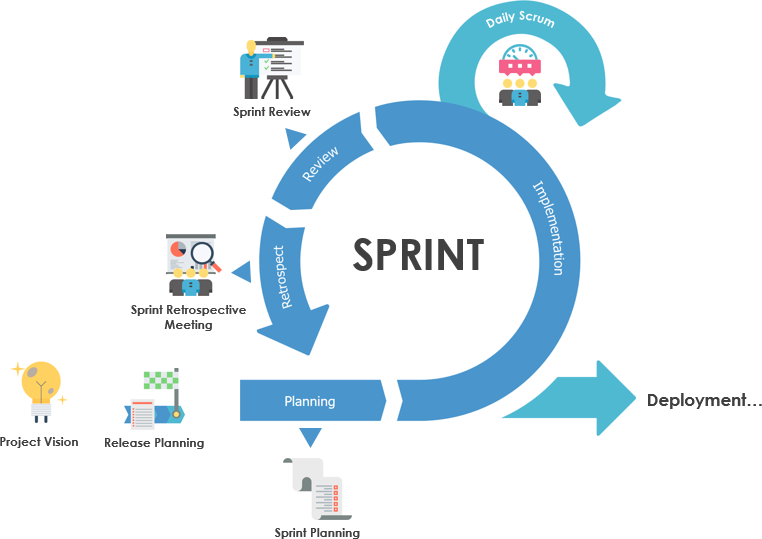
\includegraphics[width=0.5\columnwidth]{scrum}
		\caption{Metodo Scrum}
	\end{center}
\end{figure}
La situazione di emergenza sanitaria ancora non conclusa mi ha portato a vivere un'esperienza lavorativa diversa dai colleghi degli anni precedenti, infatti ha fatto sì che lo stage fosse organizzato in modalità mista: in parte da remoto ed in parte in azienda (di solito uno o due giorni alla settimana). A causa di ciò non ho potuto vivere appieno questo modello di sviluppo vista l'impossibilità di essere sempre presente in azienda. Per questo motivo il giorno concordato con i colleghi stagisti ed il tutor aziendale per andare in azienda è stato sfruttato per fare un daily scrum alternativo data la sua cadenza settimanale.\\ 
Nonostante l'emergenza sanitaria ancora in corso ho potuto comunque constatare l’efficacia e la funzionalità di questo modello di sviluppo, soprattutto per un progetto software in evoluzione quale è stato quello a cui ho lavorato.\\

\subsection{Organizzazione del lavoro}

\subsubsection{Trello}

Trello è una piattaforma online tramite la quale si può gestire i progetti in modo semplice, gratuito e flessibile. Questa piattaforma risulta essere molto utile per l'organizzazione e la gestione del workflow online.\\
Tramite questa piattaforma è possibile rappresentare le attività da svolgere in schede inserite sotto apposite colonne di avanzamento. In base a quanto si è riusciti a realizzare, è possibile spostare manualmente o automaticamente lo stato di avanzamento di ogni scheda. DA FINIRE
Per tenere traccia delle attività da svolgere è stato deciso di utilizzare la piattaforma online gestionale Trello. Tramite essa l'azienda ha creato due bacheche:
\begin{itemize}
	\item personale: disponibile solo allo stagista ed al tutor aziendale, dove sono stati inseriti i compiti decisi nel piano di lavoro suddivisi per settimana;
	\item collettiva: disponibile a tutti gli stagisti che lavorano allo stesso progetto e ai loro rispettivi tutor aziendali, dove sono state inserite le prime idee e funzionalità legate al progetto.
\end{itemize}
Nella bacheca personale sono presenti diverse schede di numero pari alle settimane di stage da svolgere mentre nella bacheca collettiva il numero delle schede dipende dal numero di funzionalità e servizi da sviluppare. 

\subsubsection{Report giornaliero}

DA FINIRE

Oltre a tenere traccia delle attività tramite Trello, l'azienda ha deciso di far scrivere allo stagista un file Excel su Drive come report giornaliero delle attività svolte. Il report era suddiviso in quattro colonne:
\begin{itemize}
	\item data: indica il giorno in è stata fatta un'attività in formato AAAA-MM-GG;
	\item descrizione: breve descrizione dell'attività svolta dal tirocinante compilata alla fine di ogni giornata lavorativa;
	\item nota: campo dove il tutor aziendale può aggiungere note di consiglio riguardo all'attività svolta, inoltre in questo campo vengono specificati i giorni festivi;
	\item spunta: casella di spunta dove il tutor indica di aver visionato l'attività svolta.
\end{itemize}

\begin{figure}[H]
	\begin{center}
		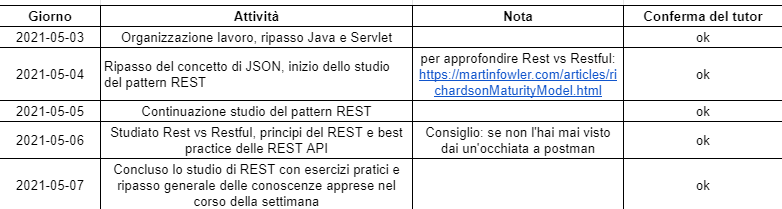
\includegraphics[width=1\columnwidth]{report}
		\caption{Spezzone del report giornaliero}
	\end{center}
\end{figure}

%**************************************************************

\subsubsection{Discord}

Per comunicare con l'intero gruppo di stagisti l'azienda ha proposto di utilizzare Discord, una piattaforma messaggistica dove noi stagisti potevamo comunicare sia con il personale aziendale che singolarmente con il proprio tutor per consigli, delucidazioni o motivi organizzativi. DA FINIRE             % Processi
% !TEX encoding = UTF-8
% !TEX TS-program = pdflatex
% !TEX root = ../tesi.tex

%**************************************************************
\chapter{Analisi dei requisiti}
\label{cap:analisi-requisiti}
%**************************************************************

\intro{In questo capitolo verranno elencati i casi d'uso delle funzionalità implementate con i relativi requisiti ed i loro tracciamento}\\

\section{Casi d'uso}
\label{sec:casi-uso}

Per lo studio dei casi d'uso del prodotto creato sono stati creati dei diagrammi.
Questi diagrammi, detti appunto dei casi d'uso (in inglese \textit{Use Case Diagram}), sono diagrammi di tipo \gls{uml} dedicati alla descrizione del sistema e delle funzioni o servizi offerti da un esso, e come gli utilizzatori interagiscono con esso.\\
Lo strumento utilizzato per la realizzazione di tali diagrammi è draw.io, piattaforma online che permette di creare diagrammi direttamente nel browser e salvarli nel proprio \textit{cloud} di \textit{Google}.

\subsection{Attori dei casi d'uso}
\label{subsec:attori}

Dopo un'attenta analisi ho concluso che per le funzionalità offerte sono presenti unicamente attori primari, in quanto non ci sono collegamenti con alcun \gls{frameworkg} o libreria esterna.
Di conseguenza i possibili attori dei casi d'uso analizzati sono i seguenti attori primari:
\begin{itemize}
	\item \textbf{utente non autenticato}: indica che l'utente non ha ancora effettuato l'autenticazione o la registrazione all'interno della \gls{web applicationg};
	\item \textbf{utente autenticato}: indica che l'utente ha effettuato l'autenticazione all'interno della \gls{web applicationg} e comporta che può accedere a diverse funzionalità che sarebbero altrimenti inaccessibili.
\end{itemize}

\begin{figure}[H] 
	\centering 
	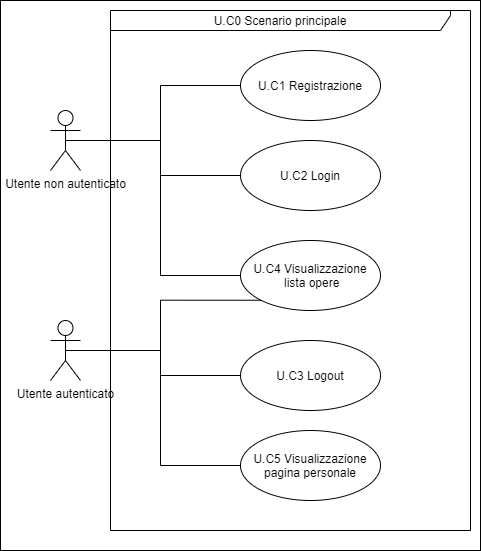
\includegraphics[width=0.8\columnwidth]{usecase/uc0} 
	\caption{U.C0 Scenario principale}
\end{figure}

\newpage

\begin{usecase}{1}{Registrazione}\label{uc1}
	\begin{figure}[H] 
		\centering 
		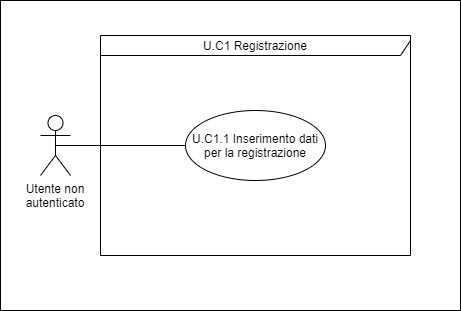
\includegraphics[width=0.7\columnwidth]{usecase/UC1} 
		\caption{U.C1 Registrazione}
	\end{figure}
\usecaseactors{Utente non autenticato.}
\usecasepre{L'utente non è ancora presente nei registri del sistema.}
\usecasedesc{L'utente accede all'applicazione e naviga fino alla pagina di registrazione. L'utente inserisce i dati necessari e li conferma, questo porta l'utente a possedere un account nel sistema.}
\usecasepost{L'utente risulta presente nei registri del sistema ed è autenticato nella piattaforma.}
\end{usecase}

\begin{usecase}{1.1}{Inserimento dati per la registrazione}\label{uc1.1}
	\begin{figure}[H] 
		\centering 
		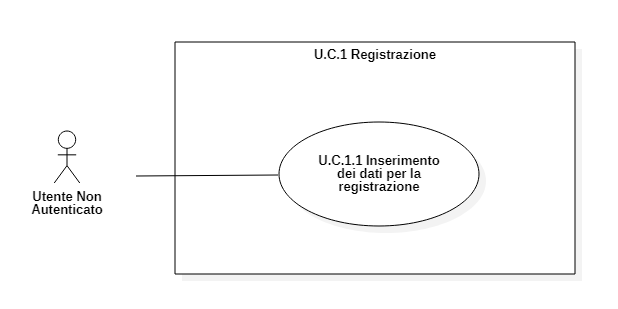
\includegraphics[width=0.9\columnwidth]{usecase/UC1.1} 
		\caption{U.C1.1 Inserimento dei dati per la registrazione}
	\end{figure}
\usecaseactors{Utente non autenticato.}
\usecasepre{L'utente non autenticato si trova nella pagina di registrazione.}
\usecasedesc{L'utente non autenticato compila i campi nel seguente modo:
\begin{itemize}
	\item Inserimento del nome (\ref{uc1.1.1});
	\item Inserimento del cognome (\ref{uc1.1.2});
	\item Inserimento dell'email (\ref{uc1.1.3});
	\item Inserimento della password (\ref{uc1.1.4});
	\item Inserimento della conferma della password (\ref{uc1.1.5});
	\item Inserimento dell'anno di nascita (\ref{uc1.1.6});
	\item Inserimento del Wallet Address (\ref{uc1.1.7}).
\end{itemize}
}
\usecasepost{L'utente ha completato la compilazione dei campi e può procedere con la registrazione.}
\end{usecase}

\begin{usecase}{1.1.1}{Inserimento del nome}\label{uc1.1.1}
\usecaseactors{Utente non autenticato.}
\usecasepre{L'utente non è autenticato e non ha compilato questo campo.}
\usecasedesc{L'utente non autenticato inserisce il proprio nome.}
\usecaseest{Viene effettuato un controllo e risulta che questo campo non è stato compilato quindi si presenta un messaggio di errore e viene fornita la possibilità di inserire nuovamente il dato (\ref{uc6}).}
\usecasepost{L'utente ha inserito il nome.}
\usecaseest{L'utente non inserisce nulla e appare il messaggio di errore.}
\end{usecase}

\begin{usecase}{1.1.2}{Inserimento del cognome}\label{uc1.1.2}
\usecaseactors{Utente non autenticato.}
\usecasepre{L'utente non è autenticato e non ha compilato questo campo.}
\usecasedesc{L'utente non autenticato inserisce il proprio cognome.}
\usecaseest{Viene effettuato un controllo e risulta che questo campo non è stato compilato quindi si presenta un messaggio di errore e viene fornita la possibilità di inserire nuovamente il dato (\ref{uc6}).}
\usecasepost{L'utente ha inserito il cognome.}
\end{usecase}

\begin{usecase}{1.1.3}{Inserimento dell'email}\label{uc1.1.3}
\usecaseactors{Utente non autenticato.}
\usecasepre{L'utente non è autenticato e non ha compilato questo campo.}
\usecasedesc{L'utente non autenticato inserisce la sua email.}
\usecaseest{
	\begin{itemize}
		\item Viene effettuato un controllo e risulta che questo campo non è stato compilato quindi si presenta un messaggio di errore e viene fornita la possibilità di inserire nuovamente il dato (\ref{uc6});
		\item Viene effettuato un controllo sul campo inserito e risulta non essere valido quindi si presenta un messaggio di errore e viene fornita la possibilità di inserire nuovamente il dato (\ref{uc7}).
	\end{itemize}
}
\usecasepost{L'utente ha inserito l'email.}
\end{usecase}

\begin{usecase}{1.1.4}{Inserimento della password}\label{uc1.1.4}
\usecaseactors{Utente non autenticato.}
\usecasepre{L'utente non è autenticato e non ha compilato questo campo.}
\usecasedesc{L'utente non autenticato inserisce la sua password.}
\usecaseest{
	\begin{itemize}
		\item Viene effettuato un controllo e risulta che questo campo non è stato compilato quindi si presenta un messaggio di errore e viene fornita la possibilità di inserire nuovamente il dato (\ref{uc6});
		\item Viene effettuato un controllo sul campo inserito e risulta non essere valido quindi si presenta un messaggio di errore e viene fornita la possibilità di inserire nuovamente il dato (\ref{uc7}).
	\end{itemize}
}
\usecasepost{L'utente ha inserito la password.}
\end{usecase}

\begin{usecase}{1.1.5}{Inserimento della conferma della password}\label{uc1.1.5}
\usecaseactors{Utente non autenticato.}
\usecasepre{L'utente non è autenticato e non ha compilato questo campo.}
\usecasedesc{L'utente non autenticato inserisce la conferma della password.}
\usecaseest{
	\begin{itemize}
		\item Viene effettuato un controllo e risulta che questo campo non è stato compilato quindi si presenta un messaggio di errore e viene fornita la possibilità di inserire nuovamente il dato (\ref{uc6});
		\item Viene effettuato un controllo sul campo inserito e risulta non essere valido quindi si presenta un messaggio di errore e viene fornita la possibilità di inserire nuovamente il dato (\ref{uc8});
		\item Viene effettuato un controllo di uguaglianza con la password precedentemente inserita e i due campi non risultano uguali quindi si presenta un messaggio di errore e viene fornita la possibilità di inserire nuovamente il dato(\ref{uc9}).
	\end{itemize}
}
\usecasepost{L'utente ha inserito la conferma della password.}
\end{usecase}

\begin{usecase}{1.1.6}{Inserimento dell'anno di nascita}\label{uc1.1.6}
\usecaseactors{Utente non autenticato.}
\usecasepre{L'utente non è autenticato e non ha compilato questo campo.}
\usecasedesc{L'utente non autenticato inserisce il proprio anno di nascita.}
\usecaseest{
	\begin{itemize}
		\item Viene effettuato un controllo e risulta che questo campo non è stato compilato quindi si presenta un messaggio di errore e viene fornita la possibilità di inserire nuovamente il dato (\ref{uc6});
		\item Viene effettuato un controllo sul campo inserito e risulta non essere valido in quanto l'utente risulta essere non maggiorenne quindi si presenta un messaggio di errore e viene fornita la possibilità di inserire nuovamente il dato (\ref{10}).
	\end{itemize}
}
\usecasepost{L'utente ha inserito l'anno di nascita.}
\end{usecase}

\begin{usecase}{1.1.7}{Inserimento del Wallet Address}\label{uc1.1.7}
\usecaseactors{Utente non autenticato.}
\usecasepre{L'utente non è autenticato e non ha compilato questo campo.}
\usecasedesc{L'utente non autenticato inserisce il Wallet Address.}
\usecaseest{
	\begin{itemize}
		\item Viene effettuato un controllo e risulta che questo campo non è stato compilato quindi si presenta un messaggio di errore e viene fornita la possibilità di inserire nuovamente il dato (\ref{uc6});
		\item Viene effettuato un controllo sul campo inserito e risulta non essere valido quindi si presenta un messaggio di errore e viene fornita la possibilità di inserire nuovamente il dato (\ref{11}).
	\end{itemize}
}
\usecasepost{L'utente ha inserito il Wallet Address.}
\end{usecase}

\begin{usecase}{2}{Login}\label{uc2}
	\begin{figure}[H] 
		\centering 
		\includegraphics[width=0.8\columnwidth]{usecase/UC2} 
		\caption{U.C2 Login}
	\end{figure}
\usecaseactors{Utente non autenticato.}
\usecasepre{L'utente non è autenticato ma è presente nei registri di sistema.}
\usecasedesc{L'utente accede all'applicazione e naviga fino alla pagina di login. L'utente inserisce i dati necessari (\ref{uc2.1}) e li conferma, questo porta l'utente ad autenticarsi nel sistema.}
\usecaseest{L'utente inserisce i dati ma non è presente nel database quindi si presenta un messaggio di errore e viene fornita la possibilità di inserire nuovamente i dati (\ref{uc12}).}
\usecasepost{L'utente risulta autenticato nella piattaforma.}
\end{usecase}

\begin{usecase}{2.1}{Inserimento dati per il login}\label{uc2.1}
	\begin{figure}[H] 
		\centering 
		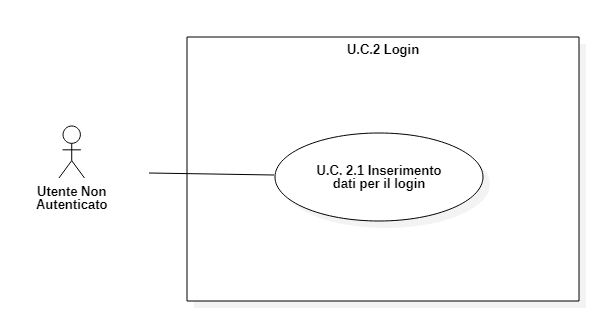
\includegraphics[width=0.8\columnwidth]{usecase/UC2.1} 
		\caption{U.C2.1 Inserimento dati per il login}
	\end{figure}
\usecaseactors{Utente non autenticato.}
\usecasepre{L'utente non autenticato si trova nella pagina di login.}
\usecasedesc{L'utente non autenticato compila i campi nel seguente modo:
\begin{itemize}
	\item Inserimento della email (\ref{uc2.1.1});
	\item Inserimento della password (\ref{uc2.1.2}).
\end{itemize}}
\usecasepost{L'utente è autenticato come utente autenticato all'interno della \gls{web applicationg}.}
\end{usecase}

\begin{usecase}{2.1.1}{Inserimento della email}\label{uc2.1.1}
\usecaseactors{Utente non autenticato.}
\usecasepre{L'utente non autenticato si trova nella pagina di login e possiede le credenziali di accesso.}
\usecasedesc{L'utente, per procedere con l'autenticazione inserisce l'email.}
\usecaseest{
	\begin{itemize}
		\item Viene effettuato un controllo e risulta che questo campo non è stato compilato quindi si presenta un messaggio di errore e viene fornita la possibilità di inserire nuovamente il dato (\ref{uc6});
		\item Viene effettuato un controllo sul campo inserito e risulta non essere valido quindi si presenta un messaggio di errore e viene fornita la possibilità di inserire nuovamente il dato (\ref{uc7}).
	\end{itemize}}
\usecasepost{L'utente ha inserito l'email.}
\end{usecase}

\begin{usecase}{2.1.2}{Inserimento della password}\label{uc2.1.2}
	\usecaseactors{Utente non autenticato.}
	\usecasepre{L'utente non autenticato si trova nella pagina di login e possiede le credenziali di accesso.}
	\usecasedesc{L'utente, per procedere con l'autenticazione inserisce la password.}
	\usecaseest{
		\begin{itemize}
			\item Viene effettuato un controllo e risulta che questo campo non è stato compilato quindi si presenta un messaggio di errore e viene fornita la possibilità di inserire nuovamente il dato (\ref{uc6});
			\item Viene effettuato un controllo sul campo inserito e risulta non essere valido quindi si presenta un messaggio di errore e viene fornita la possibilità di inserire nuovamente il dato (\ref{uc8}).
		\end{itemize}}
	\usecasepost{L'utente ha inserito la password.}
\end{usecase}

\begin{usecase}{3}{Logout}\label{uc3}
	\usecaseactors{Utente autenticato.}
	\usecasepre{L'utente è autenticato e vuole uscire dal proprio account.}
	\usecasedesc{L'utente vuole uscire dal proprio account}
	\usecasepost{L'utente non è più autenticato}
\end{usecase}

\begin{usecase}{4}{Visualizzazione lista opere}\label{uc4}
	\begin{figure}[H] 
		\centering 
		\includegraphics[width=0.8\columnwidth]{usecase/UC4} 
		\caption{U.C4 Visualizzazione lista opere}
	\end{figure}
	\usecaseactors{Utente non autenticato.}
	\usecasepre{L'utente ha aperto il sito e si trova nella pagina iniziale.}
	\usecasedesc{L'utente può visualizzare la lista delle opere in vendita. In particolare l'utente può filtrare le opere (\ref{uc4.1}) oppure visualizzare nel dettaglio un'opera selezionata (\ref{uc4.2})}
	\usecasepost{L'utente ha visualizzato la lista.}
\end{usecase}

\begin{usecase}{4.1}{Inserimento filtro sulla lista opere}\label{uc4.1}
	\usecaseactors{Utente non autenticato.}
	\usecasepre{L'utente si trova nella pagina principale e sta visualizzando le opere.}
	\usecasedesc{L'utente può applicare dei filtri alla lista di opere presenti nella homepage.}
	\usecasepost{L'utente ha visualizzato la lista di opere filtrate.}
\end{usecase}

\begin{usecase}{4.1.1}{Inserimento filtro per categorie sulla lista opere}\label{uc4.1.1}
	\usecaseactors{Utente non autenticato.}
	\usecasepre{L'utente si trova nella pagina principale e sta visualizzando le opere.}
	\usecasedesc{L'utente può applicare dei filtri per categoria alla lista di opere presenti nella homepage.}
	\usecasepost{L'utente ha visualizzato la lista di opere filtrate per categoria.}
\end{usecase}

\begin{usecase}{4.2}{Visualizzazione dettaglio opera}\label{uc4.2}
	\usecaseactors{Utente non autenticato.}
	\usecasepre{L'utente si trova nella pagina principale.}
	\usecasedesc{L'utente può selezionare un'opera per poter visualizzare le sue informazioni nel dettaglio.}
	\usecasepost{L'utente ha visualizzato i dettagli dell'opera selezionata.}
\end{usecase}

\begin{usecase}{5}{Visualizzazione pagina personale}\label{uc5}
	\begin{figure}[H] 
		\centering 
		\includegraphics[width=0.8\columnwidth]{usecase/UC5} 
		\caption{U.C5 Visualizzazione pagina personale}
	\end{figure}
	\usecaseactors{Utente autenticato.}
	\usecasepre{L'utente si trova nella home page.}
	\usecasedesc{L'utente può navigare nel sito per raggiungere la sua pagina personale.}
	\usecasepost{L'utente ha visualizzato la sua pagina.}
\end{usecase}

\begin{usecase}{5.1}{Modifica dati}\label{uc5.1}
	\begin{figure}[H] 
		\centering 
		\includegraphics[width=0.8\columnwidth]{usecase/UC5.1} 
		\caption{U.C5.1 Modifica dati}
	\end{figure}
	\usecaseactors{Utente autenticato.}
	\usecasepre{L'utente si trova nella sua pagina personale.}
	\usecasedesc{L'utente può modificare i dati personali. In dettaglio l'utente può modificare:
	\begin{itemize}
		\item il nome (\ref{uc5.1.1});
		\item il cognome (\ref{uc5.1.2});
		\item la data di nascita (\ref{uc5.1.3});
		\item l'address wallet (\ref{uc5.1.4}).
	\end{itemize}
	Per poter confermare le modifiche l'utente deve inserire la propria password (\ref{uc5.1.5})}
	\usecasepost{L'utente ha modificato i suoi dati.}
\end{usecase}

\begin{usecase}{5.1.1}{Modifica del nome}\label{uc5.1.1}
	\usecaseactors{Utente autenticato.}
	\usecasepre{L'utente è autenticato e non ha modificato questo campo.}
	\usecasedesc{L'utente può modificare il proprio nome.}
	\usecaseest{Viene effettuato un controllo e risulta che questo campo non è stato compilato quindi si presenta un messaggio di errore e viene fornita la possibilità di inserire nuovamente il dato (\ref{uc6}).}
	\usecasepost{L'utente ha modificato il nome.}
\end{usecase}

\begin{usecase}{5.1.2}{Modifica del cognome}\label{uc5.1.2}
	\usecaseactors{Utente autenticato.}
	\usecasepre{L'utente è autenticato e non ha modificato questo campo.}
	\usecasedesc{L'utente può modificare il proprio cognome.}
	\usecaseest{Viene effettuato un controllo e risulta che questo campo non è stato compilato quindi si presenta un messaggio di errore e viene fornita la possibilità di inserire nuovamente il dato (\ref{uc6}).}
	\usecasepost{L'utente ha modificato il cognome.}
\end{usecase}

\begin{usecase}{5.1.3}{Modifica della data di nascita}\label{uc5.1.3}
	\usecaseactors{Utente autenticato.}
	\usecasepre{L'utente è autenticato e non ha modificato questo campo.}
	\usecasedesc{L'utente può modificare la propria data di nascita.}
	\usecaseest{
		\begin{itemize}
			\item Viene effettuato un controllo e risulta che questo campo non è stato compilato quindi si presenta un messaggio di errore e viene fornita la possibilità di inserire nuovamente il dato (\ref{uc6});
			\item Viene effettuato un controllo sul campo inserito e risulta non essere valido in quanto l'utente risulta essere non maggiorenne quindi si presenta un messaggio di errore e viene fornita la possibilità di inserire nuovamente il dato (\ref{uc10}).
		\end{itemize}
	}
	\usecasepost{L'utente ha modificato la data di nascita.}
\end{usecase}

\begin{usecase}{5.1.4}{Modifica del wallet}\label{uc5.1.4}
	\usecaseactors{Utente autenticato.}
	\usecasepre{L'utente è autenticato e non ha modificato questo campo.}
	\usecasedesc{L'utente può modificare il proprio address wallett.}
	\usecaseest{
		\begin{itemize}
			\item Viene effettuato un controllo e risulta che questo campo non è stato compilato quindi si presenta un messaggio di errore e viene fornita la possibilità di inserire nuovamente il dato (\ref{uc6});
			\item Viene effettuato un controllo sul campo inserito e risulta non essere valido quindi si presenta un messaggio di errore e viene fornita la possibilità di inserire nuovamente il dato (\ref{uc11}).
		\end{itemize}
	}
	\usecasepost{L'utente ha modificato il proprio address wallett.}
\end{usecase}

\begin{usecase}{5.1.5}{Inserimento della password}\label{uc5.1.5}
	\usecaseactors{Utente autenticato.}
	\usecasepre{L'utente è autenticato e non ha compilato questo campo.}
	\usecasedesc{L'utente può inserire la propria password per procedere alla modifica dei dati.}
	\usecaseest{
		\begin{itemize}
			\item Viene effettuato un controllo e risulta che questo campo non è stato compilato quindi si presenta un messaggio di errore e viene fornita la possibilità di inserire nuovamente il dato (\ref{uc6});
			\item Viene effettuato un controllo sul campo inserito e risulta non essere valido quindi si presenta un messaggio di errore e viene fornita la possibilità di inserire nuovamente il dato (\ref{uc8}).
	\end{itemize}}
	\usecasepost{L'utente ha inserito la password.}
\end{usecase}

\begin{usecase}{5.2}{Visualizzazione lista opere personali}\label{uc5.2}
	\begin{figure}[H] 
		\centering 
		\includegraphics[width=0.8\columnwidth]{usecase/UC5.2} 
		\caption{U.C5.2 Visualizzazione lista opere personali}
	\end{figure}
	\usecaseactors{Utente autenticato.}
	\usecasepre{L'utente è autenticato e si trova nella sua pagina personale.}
	\usecasedesc{L'utente può visualizzare la lista delle sue opere. Inoltre ha la possibilità di visualizzare in dettaglio i dati (\ref{uc5.2.1}) oppure modificare i dati (\ref{uc5.2.2}) un'opera selezionata}
	\usecasepost{L'utente visualizza le sue opere.}
\end{usecase}

\begin{usecase}{5.2.1}{Visualizza dettaglio opera}\label{uc5.2.1}
	\usecaseactors{Utente autenticato.}
	\usecasepre{L'utente è autenticato e si trova nella pagina personale e sta visualizzando la lista delle sue opere.}
	\usecasedesc{L'utente può selezionare un'opera per poter visualizzare le sue informazioni nel dettaglio.}
	\usecasepost{L'utente ha visualizzato i dettagli dell'opera selezionata.}
\end{usecase}

\begin{usecase}{5.2.2}{Modifica opera}\label{uc5.2.2}
	\begin{figure}[H] 
		\centering 
		\includegraphics[width=0.8\columnwidth]{usecase/UC5.2.2.2} 
		\caption{U.C5.2.2 Modifica opera}
	\end{figure}
	\usecaseactors{Utente autenticato.}
	\usecasepre{L'utente è autenticato e si trova nella pagina personale e sta visualizzando la lista delle sue opere.}
	\usecasedesc{L'utente può selezionare un'opera per poter modificare i suoi dati.}
	\usecasepost{L'utente ha modificato i dati dell'opera.}
\end{usecase}

\begin{usecase}{5.2.2.1}{Modifica titolo}\label{uc5.2.2.1}
	\usecaseactors{Utente autenticato.}
	\usecasepre{L'utente è autenticato e non ha modificato questo campo.}
	\usecasedesc{L'utente può modificare il titolo dell'opera.}
	\usecaseest{Viene effettuato un controllo e risulta che questo campo non è stato compilato quindi si presenta un messaggio di errore e viene fornita la possibilità di inserire nuovamente il dato (\ref{uc6}).}
	\usecasepost{L'utente ha modificato il titolo dell'opera.}
\end{usecase}

\begin{usecase}{5.2.2.2}{Modifica descrizione}\label{uc5.2.2.2}
	\usecaseactors{Utente autenticato.}
	\usecasepre{L'utente è autenticato e non ha modificato questo campo.}
	\usecasedesc{L'utente può modificare la descrizione.}
	\usecaseest{Viene effettuato un controllo e risulta che questo campo non è stato compilato quindi si presenta un messaggio di errore e viene fornita la possibilità di inserire nuovamente il dato (\ref{uc6}).}
	\usecasepost{L'utente ha modificato la descrizione.}
\end{usecase}

\begin{usecase}{5.2.2.3}{Modifica categorie}\label{uc5.2.2.3}
	\usecaseactors{Utente autenticato.}
	\usecasepre{L'utente è autenticato e non ha modificato questo campo.}
	\usecasedesc{L'utente può modificare le categorie.}
	\usecaseest{Viene effettuato un controllo e risulta che questo campo non è stato compilato quindi si presenta un messaggio di errore e viene fornita la possibilità di inserire nuovamente il dato (\ref{uc6}).}
	\usecasepost{L'utente ha modificato le categorie.}
\end{usecase}

\begin{usecase}{5.2.2.4}{Modifica prezzo}\label{uc5.2.2.4}
	\usecaseactors{Utente autenticato.}
	\usecasepre{L'utente è autenticato e non ha modificato questo campo.}
	\usecasedesc{L'utente può modificare il prezzo.}
	\usecaseest{Viene effettuato un controllo e risulta che questo campo non è stato compilato quindi si presenta un messaggio di errore e viene fornita la possibilità di inserire nuovamente il dato (\ref{uc6}).}
	\usecasepost{L'utente ha modificato il prezzo.}
\end{usecase}

\begin{usecase}{5.3}{Upload di una nuova opera}\label{uc5.3}
	\begin{figure}[H] 
		\centering 
		\includegraphics[width=0.8\columnwidth]{usecase/UC5.3} 
		\caption{U.C5.3 Upload di una nuova opera}
	\end{figure}
	\usecaseactors{Utente autenticato.}
	\usecasepre{L'utente è autenticato e si trova nella schermata di caricamento dell'opera.}
	\usecasedesc{L'utente ha la possibilità di caricare una nuova opera.}
	\usecasepost{L'utente ha caricato una nuova opera.}
\end{usecase}

\begin{usecase}{5.3.1}{Inserimento del titolo}\label{uc5.3.1}
	\usecaseactors{Utente autenticato.}
	\usecasepre{L'utente è autenticato e non ha compilato questo campo.}
	\usecasedesc{L'utente ha la possibilità di inserire il titolo dell'opera.}
	\usecaseest{Viene effettuato un controllo e risulta che questo campo non è stato compilato quindi si presenta un messaggio di errore e viene fornita la possibilità di inserire nuovamente il dato (\ref{uc6}).}
	\usecasepost{L'utente ha inserito il titolo dell'opera.}
\end{usecase}

\begin{usecase}{5.3.2}{Inserimento della descrizione}\label{uc5.3.2}
	\usecaseactors{Utente autenticato.}
	\usecasepre{L'utente è autenticato e non ha compilato questo campo.}
	\usecasedesc{L'utente ha la possibilità di inserire la descrizione dell'opera.}
	\usecaseest{Viene effettuato un controllo e risulta che questo campo non è stato compilato quindi si presenta un messaggio di errore e viene fornita la possibilità di inserire nuovamente il dato (\ref{uc6}).}
	\usecasepost{L'utente ha inserito la descrizione.}
\end{usecase}

\begin{usecase}{5.3.3}{Inserimento del file}\label{uc5.3.3}
	\usecaseactors{Utente autenticato.}
	\usecasepre{L'utente è autenticato e non ha compilato questo campo.}
	\usecasedesc{L'utente ha la possibilità di inserire il file.}
	\usecaseest{Viene effettuato un controllo e risulta che questo campo non è stato compilato quindi si presenta un messaggio di errore e viene fornita la possibilità di inserire nuovamente il dato (\ref{uc6}).}
	\usecasepost{L'utente ha inserito il file.}
\end{usecase}

\begin{usecase}{5.3.4}{Inserimento delle categorie}\label{uc5.3.4}
	\usecaseactors{Utente autenticato.}
	\usecasepre{L'utente è autenticato e non ha compilato questo campo.}
	\usecasedesc{L'utente ha la possibilità di inserire le categorie.}
	\usecaseest{Viene effettuato un controllo e risulta che questo campo non è stato compilato quindi si presenta un messaggio di errore e viene fornita la possibilità di inserire nuovamente il dato (\ref{uc6}).}
	\usecasepost{L'utente ha inserito le categorie.}
\end{usecase}

\begin{usecase}{5.3.5}{Inserimento del prezzo}\label{uc5.3.5}
	\usecaseactors{Utente autenticato.}
	\usecasepre{L'utente è autenticato e non ha compilato questo campo.}
	\usecasedesc{L'utente ha la possibilità di inserire il prezzo.}
	\usecaseest{Viene effettuato un controllo e risulta che questo campo non è stato compilato quindi si presenta un messaggio di errore e viene fornita la possibilità di inserire nuovamente il dato (\ref{uc6}).}
	\usecasepost{L'utente ha inserito il prezzo.}
\end{usecase}

\begin{usecase}{6}{Errore campo obbligatorio}\label{uc6}
	\usecaseactors{Utente autenticato o utente non autenticato.}
	\usecasepre{L'utente non ha inserito alcun carattere in un campo dati obbligatorio.}
	\usecasedesc{L'utente non ha inserito alcun carattere in un campo dati obbligatorio e viene informato del mancato riempimento del campo dati.}
	\usecasepost{All'utente viene mostrato un messaggio che lo avvisa del mancato riempimento del campo dati obbligatorio.}
\end{usecase}

\begin{usecase}{7}{Errore email non valida}\label{uc7}
	\usecaseactors{Utente autenticato o utente non autenticato.}
	\usecasepre{L'utente ha inserito l'email in un formato non valido.}
	\usecasedesc{L'utente ha inserito l'email in un formato non valido e viene informato del scorretto inserimento del campo dati.}
	\usecasepost{All'utente viene mostrato un messaggio che lo avvisa dello scorretto formato del campo appena inserito.}
\end{usecase}

\begin{usecase}{8}{Errore password non valida}\label{uc8}
	\usecaseactors{Utente autenticato o utente non autenticato.}
	\usecasepre{L'utente ha inserito una password in un formato non valido.}
	\usecasedesc{L'utente ha inserito la password in un formato non valido e viene informato del scorretto inserimento del campo dati.}
	\usecasepost{All'utente viene mostrato un messaggio che lo avvisa dello scorretto formato del campo appena inserito.}
\end{usecase}

\begin{usecase}{9}{Errore conferma password differente}\label{uc9}
	\usecaseactors{Utente autenticato o utente non autenticato.}
	\usecasepre{L'utente ha compilato}
	\usecasedesc{L'utente ha inserito la conferma della password differente dalla password precedentemente inserita e viene informato del scorretto inserimento del campo dati.}
	\usecasepost{All'utente viene mostrato un messaggio che lo avvisa della differenza tra le due password inserite.}
\end{usecase}

\begin{usecase}{10}{Errore maggiore età}\label{uc10}
	\usecaseactors{Utente autenticato o utente non autenticato.}
	\usecasepre{L'utente ha inserito una data di nascita non valida in quanto non risulta essere maggiorenne.}
	\usecasedesc{L'utente ha inserito una data di nascita non valida in quanto non risulta essere maggiorenne e viene informato del scorretto inserimento del campo dati.}
	\usecasepost{All'utente viene mostrato un messaggio che lo avvisa dello scorretto formato del campo appena inserito.}
\end{usecase}

\begin{usecase}{11}{Errore wallet non valido}\label{uc11}
	\usecaseactors{Utente autenticato o utente non autenticato.}
	\usecasepre{L'utente ha inserito un address wallet in un formato non valido.}
	\usecasedesc{L'utente ha inserito un address wallet in un formato non valido e viene informato del scorretto inserimento del campo dati.}
	\usecasepost{All'utente viene mostrato un messaggio che lo avvisa dello scorretto formato del campo appena inserito.}
\end{usecase}

\begin{usecase}{12}{Errore utente non presente nel database}\label{uc12}
	\usecaseactors{Utente autenticato o utente non autenticato.}
	\usecasepre{L'utente ha compilato correttamente i campi ed ha inviato la richiesta al database.}
	\usecasedesc{L'utente ha compilato correttamente i campi ed ha inviato la richiesta al database ma viene effettuato un controllo e risulta non essere presente nel database, quindi viene informato l'utente dell'errore.}
	\usecasepost{All'utente viene mostrato un messaggio che lo avvisa della non corrispondenza nel database.}
\end{usecase}

\section{Tracciamento dei requisiti}
\label{bsec:tracciamento-requisiti}

Come risultato di un'attenta analisi dei requisiti e i relativi casi d'uso effettuata sul progetto sono stati individuati diversi requisiti. Questi sono stati suddivisi per classificazione e tipologia, per questo motivo si utilizza un codice identificativo per distinguerli che è così strutturato:
\begin{center}
	\textbf{R[classificazione][tipologia][codice]}
\end{center}
La descrizione del codice è la seguente:
\begin{itemize}
	\item \textbf{R}: acronimo per Requisito;
	\item \textbf{classificazione}: individua la classificazione del requisito e può essere:
	\begin{itemize}
		\item [F =] funzionale
		\item [Q =] qualitativo
		\item [V =]  di vincolo
	\end{itemize}
	\item \textbf{tipologia}: individua la tipologia del requisito e può essere:
	\begin{itemize}
		\item [O =] obbligatorio
		\item [D =] desiderabile
		\item [F =] facoltativo
	\end{itemize}
\end{itemize}

Nelle sezioni seguenti sono riassunti i requisiti ed il loro tracciamento con i casi d'uso delineati in fase di analisi.

\begin{table}[H]
\caption{Tabella del tracciamento dei requisti funzionali}
\label{tab:requisiti-funzionali}
\renewcommand{\arraystretch}{1.6}
\begin{tabularx}{\textwidth}{lXl}
\hline\hline
\textbf{Requisito} & \textbf{Descrizione} & \textbf{Fonte}\\
\hline
RFO1 & L'utente non autenticato può effettuare la registrazione al sito & UC1 \\
\hline
RFO1.1 & L'utente non autenticato inserisce i dati per la registrazione & UC1.1 \\
\hline
RFO1.1.1 & L'utente non autenticato inserisce il nome & UC1.1.1 \\
\hline
RFO1.1.2 & L'utente non autenticato inserisce il cognome & UC1.1.2 \\
\hline
RFO1.1.3 & L'utente non autenticato inserisce l'email & UC1.1.3 \\
\hline
RFO1.1.4 & L'utente non autenticato inserisce la password & UC1.1.4 \\
\hline
RFO1.1.5 & L'utente non autenticato inserisce la conferma della password & UC1.1.5 \\
\hline
RFO1.1.6 & L'utente non autenticato inserisce l'anno di nascita & UC1.1.6 \\
\hline
RFO1.1.7 & L'utente non autenticato inserisce il Wallett Address & UC1.1.7 \\
\hline
RFO2 & L'utente non autenticato può effettuare il login al sito & UC2 \\
\hline
RFO2.1 &L'utente non autenticato inserisce i dati per il login & UC2.1 \\
\hline
RFO2.1.1 & L'utente non autenticato inserisce l'email & UC2.1.1 \\
\hline
RFO2.1.2 & L'utente non autenticato inserisce  la password & UC2.1.2 \\
\hline
RFO3 & L'utente autenticato può effettuare il logout & UC3 \\
\hline
RFO4 & L'utente autenticato o non autenticato può visualizzare la lista delle opere nella homepage & UC4 \\
\hline
RFO4.1 & L'utente autenticato o non autenticato può applicare dei filtri sulla lista delle opere & UC4.1 \\
\hline
RFO4.1.1 & L'utente autenticato o non autenticato può applicare dei filtri per categorie sulla lista delle opere & UC4.1.1 \\
\hline
RFO4.2 & L'utente autenticato o non autenticato può visualizzare in dettaglio l'opera selezionata & UC4.2 \\
\hline
RFO5 & L'utente autenticato può visualizzare la sua pagina personale & UC5 \\
\hline
RFO5.1 & L'utente autenticato può modificare i suoi dati & UC5.1 \\
\hline
RFO5.1.1 & L'utente autenticato può modificare il suo nome & UC5.1.1 \\
\hline
RFO5.1.2 & L'utente autenticato può modificare il suo cognome & UC5.1.2 \\
\hline
RFO5.1.3 & L'utente autenticato può modificare la sua data di nascita & UC5.1.3 \\
\hline
RFO5.1.4 & L'utente autenticato può modificare il suo address wallet & UC5.1.4 \\
\hline
RFO5.1.5 & L'utente autenticato può inserire la password per confermare le modifiche effettuate & UC5.1.5 \\
\hline
RFO5.2 & L'utente autenticato può visualizzare le sue opere personali & UC5.2 \\
\hline
RFO5.2.1 & L'utente autenticato può visualizzare in dettaglio l'opera selezionata  & UC5.2.1 \\
\hline
\end{tabularx}
\end{table}%

\begin{table}[H]
\caption{Continuazione della tabella del tracciamento dei requisti funzionali}
\label{tab:requisiti-funzionali1}
\renewcommand{\arraystretch}{1.6}
\begin{tabularx}{\textwidth}{lXl}
\hline\hline
RFO5.2.2 & L'utente autenticato può modificare l'opera selezionata & UC5.2.2 \\
\hline
RFO5.2.2.1 & L'utente autenticato può modificare il titolo dell'opera & UC5.2.2.1 \\
\hline
RFO5.2.2.2 & L'utente autenticato può modificare la descrizione dell'opera & UC5.2.2.2 \\
\hline
RFO5.2.2.3 & L'utente autenticato può modificare le categorie dell'opera & UC5.2.2.3 \\
\hline
RFO5.2.2.4 & L'utente autenticato può modificare il prezzo dell'opera & UC5.2.2.4 \\
\hline
RFO5.3 & L'utente autenticato può caricare una nuova opera & UC5.3 \\
\hline
RFO5.3.1 & L'utente autenticato può inserire il titolo & UC5.3.1 \\
\hline
RFO5.3.2 & L'utente autenticato può inserire la descrizione & UC5.3.2 \\
\hline
RFO5.3.3 & L'utente autenticato può inserire il file & UC5.3.3 \\
\hline
RFO5.3.4 & L'utente autenticato può inserire le categorie & UC5.3.4 \\
\hline
RFO5.3.5 & L'utente autenticato può inserire il prezzo & UC5.3.5 \\
\hline
\end{tabularx}
\end{table}%

\begin{table}[H]
\caption{Tabella del tracciamento dei requisiti qualitativi}
\label{tab:requisiti-qualitativi}
\renewcommand{\arraystretch}{1.6}
\begin{tabularx}{\textwidth}{lXl}
\hline\hline
\textbf{Requisito} & \textbf{Descrizione} & \textbf{Fonte}\\
\hline
RQO1 & Il codice sorgente prodotto deve essere disponibile in una repository pubblica su Github & Interna \\
\hline
RQ02 & Deve essere prodotto un documento tecnico che spieghi il funzionamento del codice prodotto & Interna \\
\hline
\end{tabularx}
\end{table}%

\begin{table}[H]
\caption{Tabella del tracciamento dei requisiti di vincolo}
\label{tab:requisiti-vincolo}
\renewcommand{\arraystretch}{1.6}
\begin{tabularx}{\textwidth}{lXl}
\hline\hline
\textbf{Requisito} & \textbf{Descrizione} & \textbf{Fonte}\\
\hline
RVO1 & Le maschere devono essere sviluppate tramite il framework Vue.js & Interna \\
\hline
RVO2 & Le maschere devono essere sviluppate tramite il linguaggio javascript & Interna \\
\hline
\end{tabularx}
\end{table}%             % Concept Preview
% !TEX encoding = UTF-8
% !TEX TS-program = pdflatex
% !TEX root = ../tesi.tex

%**************************************************************
\chapter{Progettazione e codifica}
\label{cap:progettazione-codifica}
%**************************************************************

\intro{In questo capitolo verranno spiegate le tecnologie utilizzate per lo sviluppo e l'architettura del prodotto software}\\

%**************************************************************
\section{Tecnologie e strumenti}
\label{sec:tecnologie-strumenti}

Di seguito viene data una panoramica delle tecnologie e strumenti utilizzati per lo sviluppo delle maschere e per la collaborazione con i colleghi stagisiti ed il tutor aziendale.

\subsection{Tecnologie}

\subsubsection*{Vue.js}
\begin{figure}[H]
	\begin{center}
		
\includegraphics[width=0.7\columnwidth]{vue.png}
		\caption{Logo di Vue.js}
	\end{center}
\end{figure}
Vue.js è un framework javascript open source nato nel 2013 che presenta un'architettura adottabile in modo incrementale che si concentra sulla composizione dei componenti, inoltre sono presenti funzionalità avanzate offerte tramite librerie e pacchetti di supporto. I componenti Vue estendono gli elementi HTML di base per incapsulare del codice riutilizzabile quindi a livello generale i componenti sono elementi personalizzati a cui il compilatore Vue associa una particolare funzionalità.\\
Vue utilizza quindi una sintassi basata su HTML e consente di associare il DOM renderizzato ai dati dell'istanza di Vue sottostante. In questo modo i modelli Vue possono essere analizzati da browser e parser HTML conformi alle modifiche ed inoltre con il sistema di reattività Vue è in grado di calcolare il numero minimo di componenti per eseguire nuovamente il rendering applicando la quantità minima di manipolazioni DOM quando cambia lo stato dell'app. Vue presenta un sistema reattivo grazie all'utilizzo di oggetti semplici Javascript ed ad un re-rendering ottimizzato: ogni componente durante il render tiene traccia delle sue dipendenze in modo tale che il sistema sappia quando e di quali componenti deve effettuare nuovamente il render.\\
Un problema che afflige le web application a pagina singola è che quest'ultime forniscono agli utenti la risposta basata solamente sull'URL dal server, di conseguenza l'utilizzo dei segnalibri a determinate schermate e la condivisione dei collegamenti a sezioni specifiche risulta molto difficile se non impossibile. Vue.js per riuscire a risolvere questo problema fornisce un'interfaccia, detta router, che da la possibilità di modificare ciò che viene visualizzato sulla pagina in base all'URL indipendentemente da come esso viene modificato. Infatti Vue.js viene fornito con il pacchetto open source "vue-router" che fornisce un'API per aggiornare l'URL dell'applicazione, supportare la cronologia di navigazione e le reimpostazioni di email e password. Tramite questa tipologia di router i componenti devono essere mappati alla route a cui appartengono per indicare dove deve essere eseguito il loro render.\\
Questo framework implementa il pattern MVVM, acronimo per Model-View-View-Model, una declinazione del più famoso MVC, ovvero Model-View-Controller. I componenti del MVVM sono:
\begin{itemize}
	\item Model (o Modello): l'implementazione del dominio dati come per il classico Modello del pattern MVC;
	\item View (o Vista): il componente grafico renderizzato dall'utente formato da HTML e CSS;
	\item ViewModel (o Vista per il Modello): il collante tra gli altri due componenti, esso fornisce alla View i dati in formato consono alla rappresentazione ed il comportamento di alcuni elementi dinamici.
\end{itemize}
La grossa differenza tra il pattern implementato da Vue.js e il Model-View-Controller sta nella differenza tra Controller e ViewModel. Il primo, infatti, è una porzione di codice che gestisce la logica di business grazie al Model e ritorna una View da mostrare all'utente; il secondo, invece, rappresenta una versione parallela al Model che risulta essere legato alla View e descrive il comportamento di quest'ultima con funzioni associate. Quindi mentre il Controller esegue logiche di business prima del rendering della View, il ViewModel definisce il comportamento dell'applicazione a runtime.

\subsubsection*{Vuetify}
Vuetify è un framework UI completo costruito su Vue.js nel 2014 ed il suo obiettivo è fornire agli sviluppatori gli strumenti per poter creare esperienze utente ricche e coinvolgenti. A differenza di altri framework Vuetify è progettato da zero in modo tale da renderlo facile da imparare ed essere gratificante da padroneggiare con centinaia di componenti realizzate dalle specifiche di Material Design.\\
Un pregio di questo framework è che adotta un approccio al mobile, questo significa che la web application sviluppata tramite esso sarà pienamente utilizzabile immediatamente su un tablet, un telefono ed un computer. Inoltre è un framework in sviluppo attivo che viene aggiornato settimanalmente rispondendo ai problemi e relativi report della community. Un altro pregio è, come si può vedere nell'immagine sottostante, il gran numero di funzionalità che possiede Vuetify in confronto agli altri framework di Vue.
\begin{figure}[H]
	\begin{center}
		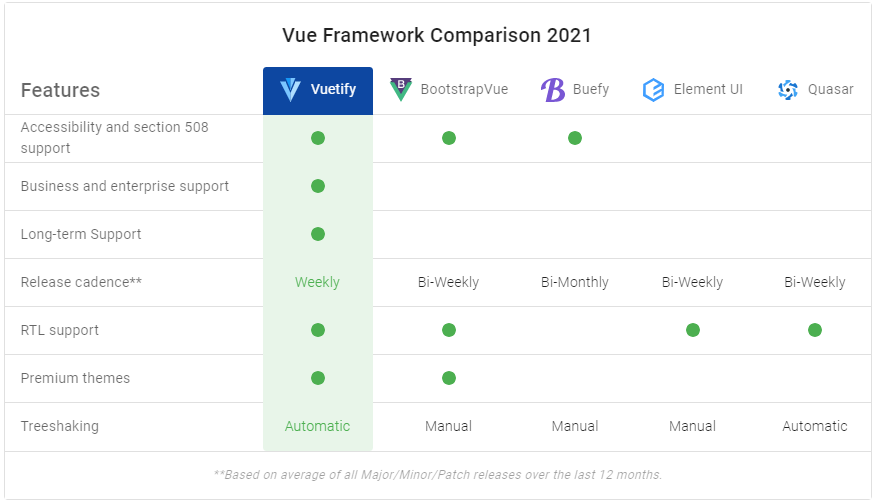
\includegraphics[width=1\columnwidth]{vuetify.png}
		\caption{Funzionalità di Vuetify}
	\end{center}
\end{figure}

\subsection{Strumenti}

\subsubsection{Github}

Github è un servizio web e cloud-based fondato nel 2008 che aiuta gli sviluppatori ad archiviare, gestire il codice, tracciare e controllare le modifiche. I due argomenti principali legati a Github sono: controllo versioni e Git.\\
Il controllo versioni aiuta a tracciare e gestire le modifiche del codice di un progetto software: più un progetto risulta essere di grandi dimensioni più il controllo delle versioni diventa fondamentale. Infatti questo aiuta gli sviluppatori a lavorare con sicurezza attraverso due azioni:
\begin{itemize}
	\item branching: uno sviluppatore duplica parte del codice sorgente, detto repository, in modo da apportare modifiche in modo sicuro senza influenzare l'intero progetto;
	\item merging: una volta che lo sviluppatore è certo di aver prodotto del codice funzionante può fondere quel codice nel quello sorgente e renderlo ufficiale.
\end{itemize}
In questo modo tutte le modifiche possono essere monitorate e, se necessario, ripristinate. Inoltre grazie a questi concetti è possibile lavorare sullo stesso progetto in diversi sviluppatori senza problemi di ripetizioni di codice o conflitti durante lo sviluppo.\\
Git è un sistema di controllo verisoni distribuito realizzato nel 2005, ovvero l'intero codice base e la cronologia sono disponibili sul computer di ogni sviluppatore. In questo modo è possibile creare facilmente ramificazioni e fusioni.

\subsubsection{Figma}

Figma è uno strumento nato nel 2016 rivolto ai web designer che hanno bisogno di un tool per la progettazione di interfacce. I vantaggi offerti da questo strumento sono i seguenti:
\begin{itemize}
	\item accessibilità multipiattaforma
	\item sistema di collaborazione in real-time
	\item utilizzo degli strumenti responsive oriented per una progettazione ottimale
	\item lavora in vettoriale
\end{itemize}
Grazie a questo strumento io e gli altri stagisti legati all'ambito front end abbiamo potuto creare dei prototipi delle maschere che avremmo dovuto sviluppare.

\subsubsection{Stoplight}

Stoplight è una piattaforma di progettazione \gls{api} collaborativa che si integra perfettamente nei flussi di lavoro per consentire a chiunque lavori con le \gls{api} di essere più produttive. Questa piattaforma si basa su tre principi guida fondamentali, in modo da essere responsabili, collaborativi e con intenti positivi. I principi sono i seguenti:
\begin{itemize}
	\item quando si vede un'opportunità per avere un impatto, bisogna coglierla;
	\item bisogna confidare l'uno nell'altro per aggiungere valore e risolvere problemi attraverso il lavoro di squadra;
	\item bisogna cercare di capire gli altri ascoltando, indagando e rispondendo con attenzione.
\end{itemize}
Grazie a questa piattaforma si può aiutare gli utenti interni ed esterni ad integrarsi rapidamente alll'\gls{api} di un altro utente pubblicando documentazione interattiva, tutorial ed esempi di codice sempre aggiornati.

\subsubsection{Visual Studio Code}

%**************************************************************
\section{Ciclo di vita del software}
\label{sec:ciclo-vita-software}

%**************************************************************
\section{Progettazione}
\label{sec:progettazione}

\subsubsection{Namespace 1} %**************************
Descrizione namespace 1.

\begin{namespacedesc}
    \classdesc{Classe 1}{Descrizione classe 1}
    \classdesc{Classe 2}{Descrizione classe 2}
\end{namespacedesc}


%**************************************************************
\section{Design Pattern utilizzati}

%**************************************************************
\section{Codifica}
             % Product Prototype
% !TEX encoding = UTF-8
% !TEX TS-program = pdflatex
% !TEX root = ../tesi.tex

%**************************************************************
\chapter{Verifica e validazione}
\label{cap:verifica-validazione}
%**************************************************************

\textit{In questo capitolo verranno descritti gli strumenti e i processi utilizzati per la verifica del codice.}

\section{Strumenti per la verifica}
\label{sec:strumenti-per-verifica}

Per verificare il codice prodotto ho utilizzato la libreria ufficiale di test \textit{Vue Test Utils}. Grazie a questa libreria si possono testare le interazioni dell'utente, come un click di un bottone, le chiamate al \gls{back endg}, le \textit{routes} e l'utilizzo di Vuex.

\section{Verifica}
\label{sec:verifica}

Per ogni componente ho creato un file che, nella fase di \textit{run}, viene chiamato \textit{test suit}. Ogni \textit{text suit} può contenere al suo interno diversi test.
\begin{lstlisting}[caption=Esempio di test-Pagina di login., label=lst::esTest]
	describe('login.vue', () => {
		let vuetify;
		beforeEach(() => {
			vuetify = new Vuetify();
		});
		const wrapper = shallowMount(login, {
			localVue,
			store,
			vuetify
		});
		it('Check if content render', () => {
			expect(wrapper.contains('v-container')).toBe(true);
		});
		it('Check if button is disabled with empty fields', ()=> {
			const email="";
			const password="";
			
			var emailInput = wrapper.find('#emailInput');
			emailInput.element.value = email;
			var passwordInput = wrapper.find('#passwordInput');
			passwordInput.element.value = password;
			
			expect(wrapper.vm.isFormValid).toBeFalsy();
			expect(wrapper.find('v-btn').element.hasAttribute('disabled')).not.toBe(true);
		});
		it('Check if email is changed after user interaction', () =>{
			var emailInput = wrapper.find('#emailInput');
			wrapper.find('#emailInput').trigger('click');
			wrapper.find('#emailInput').trigger('input');
			expect(emailInput.value).not.toBe('');
		});
		it('Check if old password is changed after user interaction', () =>{
			var passwordInput = wrapper.find('#passwordInput');
			wrapper.find('#passwordInput').trigger('click');
			wrapper.find('#passwordInput').trigger('input');
			expect(passwordInput.value).not.toBe('');
		});
	});
\end{lstlisting}
Prendiamo come esempio lo \textit{snippet} di codice soprastante che è il \textit{test suit} per la pagina di login.
Per prima cosa viene effettuato il \textit{mock} del componente tramite il comando \textit{shallowMount} dove vengono anche specificati i vari \textit{plugin} e lo \textit{store} utilizzati. Ogni \textit{it} presente nel codice rappresenta un singolo test.\\
Il primo test che ho effettuato è il controllo che la pagina renderizzi correttamente i suoi contenuti.
I controlli successivi che ho effettuato sono invece legati all'interazione dell'utente con gli elementi presenti nella pagina. I controlli che eseguo sono ad esempio che il bottone sia disabilitato se l'utente non compila correttamente tutti i campi della \textit{form}, oppure che i campi della \textit{form} vengano compilati dopo l'interazione dell'utente.\\
Per ogni componente ho effettuato test analoghi a quello appena descritto.

\section{Validazione e collaudo}

Infine durante le ultime settimane ho effettuato in collaborazione con un collega stagista l'integrazione al \gls{back endg} risolvendo possibili bug dovuti alle incongruenze tra il \gls{back endg} effettivo e quello simulato tramite stoplight.\\
Inoltre ho prodotto il documento tecnico richiesto dall'azienda riguardante il mio lavoro in modo che chiunque arrivi a prendere in mano il mio codice possa capire la logica che regge il mio lavoro.\\
Infine io e gli altri stagisti che hanno svolto lo stage nello stesso periodo abbiamo preparato una breve presentazione con demo effettiva del lavoro svolto da mostrare l'ultimo giorno a tutti i dipendenti disponibili dell'azienda.
             % Product Design Freeze e SOP
% !TEX encoding = UTF-8
% !TEX TS-program = pdflatex
% !TEX root = ../tesi.tex

%**************************************************************
\chapter{Nozioni apprese}
\label{cap:nozioni-apprese}
%**************************************************************

\intro{In questo capitolo verranno elencate e spiegate brevemente le nozioni apprese durante questo percorso di stage.}

%**************************************************************
\section{Organizzazione dello studio}

Come precedentemente spiegato le ore complessive dello stage possono essere considerate suddivise in 3 periodi:
\begin{itemize}
	\item periodo di studio della durata di circa 160 ore;
	\item periodo di sviluppo della durata di circa 120 ore;
	\item peridio di convalidazione finale della durata di circa 40 ore.
\end{itemize}
Le prime nozioni mi sono maggiormente servite per poter sviluppare le maschere, mentre le seconde mi sono servite per conoscenza generale e migliore collaborazione con i colleghi addetti al reparto back end.

%**************************************************************
\section{Nozioni principali}

\subsection{Javascript}

Javascript è un linguaggio di programmazione orientato agli oggetti e agli eventi comunemente utilizzato per la programmazione Web lato client. La sua enorme diffusione è dovuta al gran numero di librerie nate per semplificare la programmazione sul browser, dalla nascita di \gls{frameworkg} lato server e il mondo mobile che lo supporta come linguaggio principale.\\
La caratteristica principale di Javascript è quella di essere il linguaggio di \textit{scripting} per eccellenza e questo comporta una serie di vantaggi e svantaggi secondo l'uso che se ne deve fare e considerando il rapporto che si instaura nel meccanismo client-server. Il server invia al \textit{client} i dati che possono arrivare in due diversi formati (testo e binario), ma il \textit{client} sa comprendere solo il formato binario, per cui se arrivano dati in quel formato diventeranno immediatamente eseguibili altrimenti il \textit{client} dovrà interpretare i dati.\\
Sono presenti numerosi vantaggi e svantaggi di questo linguaggio, più importanti da sapere sono i seguenti:
\begin{itemize}
	\item \textbf{Vantaggi}:
	\begin{itemize}
		\item Velocità: è un linguaggio veloce, siccome ogni funzione può essere avviata immediatamente invece di dover contattare il server ed aspettare una sua risposta;
		\item Semplicità: è un linguaggio relativamente semplice da imparare ed implementare;
		\item Versatilità: è un linguaggio che lavora bene con altri linguaggi e può essere usato in una grande varietà di applicazioni, infatti può essere inserito in una pagina web indipendentemente dall'estensione del file e può essere utilizzato all'interno di script scritti in altri linguaggi;
		\item Carico del server: essendo Javascript un linguaggio lato client questo fa ridurre le domande al server del sito web.
	\end{itemize}
	\item \textbf{Svantaggi}:
	\begin{itemize}
		\item Sicurezza: visto che il codice si esegue nel computer dell'utente può essere sfruttato per scopi dannosi;
		\item Affidamento all'utente finale: gli script lato server producono sempre lo stesso risultato ma gli script lato client possono risultare imprevedibili perché possono essere interpretati in maniera differente in base al browser utilizzato. Questo difetto però può essere mitigato provando il proprio codice sui browser più utilizzati dagli utenti.
	\end{itemize}
\end{itemize}

\subsection{Vue.js}

Vue.js è un \gls{frameworkg} javascript open-source per la configurazione di interfacce utente e single-page application.\\

\textit{Questo framework verrà spiegato nel dettaglio nel capitolo riguardante la Progettazione e codifica.}

%**************************************************************
\section{Nozioni secondarie}

\subsection{Java}

Java è un linguaggio di programmazione ad alto livello, orientato agli oggetti e a tipizzazione statica che si appoggia sull'omonima piattaforma software di esecuzione. Java nasce dall'esigenza di risolvere due problemi concreti comuni tra i linguaggi orientati ad oggetti: garantire maggiore semplicità nella scrittura e gestione del codice, e permettere la realizzazione di programmi slegati da un'architettura precisa.\\
Il primo problema fu risolto utilizzando un sistema basato sulla gestione della memoria detto \textit{garbage collector}, liberando così il programmatore dall'onere della gestione della memoria. Il secondo problema, invece, fu risolto facendo in modo che i programmi non fossero compilati in codice macchina ma in una sorta di codice intermedio che dovrà poi essere eseguito non dall'hardware direttamente ma dalla macchina virtuale detta JVM, ovvero \textit{Java Virtual Machine}.\\

\subsection{Concetti web}

Riguardo a questo argomento sono stati ripassati in dettaglio due argomenti: il concetto di Servlet e il concetto di REST.

\subsubsection{Servlet}

Una Servlet è un oggetto scritto in linguaggio Java in grado di gestire le richieste generate da uno o più client attraverso scambi di messaggi tra il server ed i client stessi. La servlet può utilizzare le Java API per implementare le diverse funzionalità e le specifiche servlet API per mettere a disposizione un'interfaccia standard per gestire le comunicazioni tra il web client e la servlet. E' importante sapere che le servlet non hanno delle GUI.\\
I vantaggi della Servlet sono:
\begin{itemize}
	\item \textit{efficienza}: la Servlet viene istanziata e caricata una sola volta, alla prima invocazione, mentre le chiamate successive sono gestite chiamando nuovi thread;
	\item \textit{portabilità}: le servlet possono essere facilmente programmate e "portate" in diverse piattaforme;
	\item \textit{persistenza}: dopo essere stata caricata in memoria la servlet rimane anche nelle successive richieste;
	\item \textit{gestione delle sessioni}: grazie alle servlet si riesce a superare la limitazione dei protocolli HTTP senza stati.
\end{itemize}

\subsubsection{REST}

REST è un insieme di principi architetturali per la progettazione che rendono il Web adatto a realizzare Web Service. I principi sono:
\begin{itemize}
	\item \textit{identificazione delle risorse}: per risorsa si intende qualsiasi elemento in oggetto di elaborazione, ovvero qualsiasi oggetto su cui è possibile effettuare operazioni. Ciascuna risorsa deve essere identificata univocamente, il meccanismo più naturale è il concetto di URI;
	\item \textit{uso esplicito dei metodi HTTP}: serve un meccanismo per indicare le operazioni che si possono fare sulle risorse, per questo motivo si sfruttano i metodi predefiniti del protocollo HTTP;
	\item \textit{risorse autodescrittive}: è opportuno usare i formati più standard possibili per semplificare l'interazione con il client. Il tipo di rappresentazione è indicato nella risposta HTTP;
	\item \textit{collegamenti tra risorse}: le risorse devono essere messe tra di loro in relazione tramite link ipertestuali, è un principio detto HATEOAS;
	\item \textit{comunicazione senza stato}: è un principio secondo il quale una richiesta non ha alcuna relazione con le richieste precedenti e successive.
\end{itemize}

\subsection{Spring}

Il framework Spring è una piattafroma Java che fornisce un'infrastruttura di supporto per sviluppatori in Java in modo tale che loro si occupino dalla parte dell'applicazione. I benefici di Spring sono:
\begin{itemize}
	\item dipendenze esplicite ed evidenti grazie alla Dependency Injection;
	\item i contenitori legati all'Inversion of Control tendono ad essere leggeri;
	\item non reinventa nulla, prende quello che è già esistente e lo rende disponibile;
	\item è organizzato in modo modulare quindi il programmatore si preoccupa del pacchetto che gli interessa;
	\item è un model view controller framework ben formato;
	\item fornisce un'interfaccia di gestione delle transizioni.
\end{itemize}
Di questo framework in particolare ho studiato: Spring Boot, Spring Data, Spring Data JPA e Spring Data REST. Nelle sezioni successive verranno spiegati questi concetti.

\subsubsection{Spring Boot}

Spring Boot è un progetto Spring che ha lo scopo di rendere più semplice lo sviluppo e l'esecuzione delle applicazioni Spring. Un'applicazione richiede molti metadati per la configurazione e puoi risultare pesante, Spring Boot invece alleggerisce questo meccanismo fornendo una configurazione automatica. Infatti esso è basato su opinioni e convenzioni proprie per avere una configurazione minima con la possibilità di riscriverle se necessario. Alcune caratteristiche principali sono legate ai seguenti aspetti:
\begin{itemize}
	\item \textit{starter dependencies}, ovvero configurazione automatica delle librerie e delle dipendenze;
	\item configurazione automatica di \textit{bean} e componenti e delle loro relazioni;
	\item \textit{actuator}, per ispezionare un applicazione in esecuzione.
\end{itemize} 
Spring Boot quindi semplifica la gestione delle dipendenze fornendo e supportando una serie di dipendenze dette \textit{starter}, ovvero dipendenze la cui inclusione implica l'inclusione automatica delle loro dipendenze transitive. La classe detta \textit{Spring Boot Application} esegue l'avvio dell'applicazione etichettando la classe di configurazione, abilitando la scansione e l'identificazione automatica dei componenti, ed infine creando i componenti mancanti necessari alla configurazione dell'applicazione.\\
Per riassumere i vantaggi offerti da Spring Boot sono:
\begin{itemize}
	\item possibilità di incorporare applicazioni web server per cui non è necessario l'uso di file WAR, acronimo di \textit{Web Application Archive};
	\item configurazione Maven semplificata;
	\item configurazione automatica se possibile;
	\item fornitura di caratteristiche non funzionali come metriche o configurazioni esternalizzate.
\end{itemize}

\subsubsection{Spring Data}
Spring Data è un progetto ad alto livello di Spring con lo scopo di unificare e facilitare l'accesso a diversi livelli di archiviazione, ovvero database sia relazionali che non relazionali. Spring Data fornisce interfacce generiche per gli aspetti legati a \textit{Crud Repository} e \textit{Paging And Sorting Repository} per ottenere implementazioni specifiche dall'archivio di persistenza. Grazie alle repository basterà scrivere l'interfaccia con i metodi di ricerca definiti in base ad un determinato insieme di convenzioni che possono variare in base al tipo di archiviazione in uso. Sarà Spring  a fornire un'implementazione appropriata di tale interfaccia in fase di esecuzione.

\subsubsection{Spring Data JPA}
Spring Data JPA aiuta ad implementare facilmente sistemi basati su archiviazione di tipo JPA, framework per il linguaggio di programmazione Java che gestisce la persistenza dei dati in un database relazionale che usano le Java Platform, Standard Edition e Java Enterprise Edition. Questo modulo infatti si occupa del supporto per i livelli di accesso ai dati basati su JPA e rende più semplice la creazione di applicazioni basate su Spring che utilizzano tecnologie di accesso ai dati.\\
Per molto tempo implementare un livello di accesso ai dati è risultato complicato: era necessario scrivere molto codice per eseguire \textit{query} semplici, impaginazione e controllo dei dati. Spring Data JPA mira a ridurre lo sforzo all'importo effettivamente necessario. Lo sviluppatore scriverà le interfacce del \textit{repository}, inclusi i metodi personalizzati, e sarà Spring a fornire l'implementazione automaticamente.

\subsubsection{Spring Data REST}
Spring Data REST semplifica la creazione di servizi Web REST basati su \textit{repository} di Spring Data analizzando il modello di dominio dell'applicazione ed espone le risorse HTTP basate su \textit{hypermedia} per gli aggregati contenuti nel modello.\\
Spring Data REST definisce automaticamente gli \textit{endpoint} di aggiunta, visualizzazione, rimozione e modifica. Così facendo viene eliminato molto del lavoro manuale solitamente associato a queste attività e rende semplice l'implementazione delle funzionalità \gls{CRUDg}$_G$.  

\subsection{Blockchain}

La Blockchain è una tecnologia che sfrutta le caratteristiche di una rete informatica di nodi e consente di gestire ed aggiornare, in modo univoco e sicuro, un registro contenente dati ed informazioni in maniera aperta, condivisa e distribuita senza la necessità di un'entità centrale di controllo e verifica. Le applicazioni della blockchain sono contraddistinte dalla necessità di decentralizzazione e disintermediazione in modo da evitare banche, istituzioni finanziare e così via.\\
Queste tecnologia abilita l'Internet of Value e si basa su un registro distribuito, sistema in cui i nodi di una rete possiedono la medesima copia di un database che modificano e leggono i dati indipendentemente dagli altri nodi. Il registro di queste tecnologie è strutturato come una catena di blocchi contenenti le transazioni ed il consenso è distribuito su tutti i nodi della rete, in questo modo i nodi possono partecipare al processo di validazione delle transazioni da includere nel registro.

\subsection{Ethereum}

Ethereum è una piattaforma digitale che permette di costruire una gamma di applicazioni decentralizzate. Queste applicazioni possono includere programmi di sicurezza, sistemi elettorali e metodi di pagamento. Questa piattaforma opera fuori dal mandato delle autorità centrali ed è per questo motivo che opera nel mercato delle criptovalute.\\
Ethereum funziona come piattaforma software basata sulla tecnologia blockchain, simile a quella dei bitcoin perchè conserva le transazioni, ed inoltre permette ai programmatori di costruire applicazioni decentralizzate. Queste applicazioni sono software open source che utilizzano la blockchain e gli smart contract e non hanno bisogno di mediatori. 

\subsection{NFT}

\gls{NFT}, acronimo per Non Fungible Token, si tratta di token insostituibili che rappresentano la proprietà di un bene, come un'opera d'arte digitale o reale. Un token è un oggetto con un valore particolare e simbolico, in particolare un token sulla blockchain è un'informazione digitale registrata su un registro distribuito. Questa informazione è associata ad un utente specifico e rappresenta un certo tipo di diritto, come proprietà di un oggetto o la ricezione di un pagamento. Gli \gls{NFT} sono diversi dagli altri token perchè sono insostituibili, unici, indivisibili ed è questo il motivo per cui si prestano alla cessione dei diritti di proprietà di opere d'arte.\\
Quando una persona compra un \gls{NFT} si deve capire che:
\begin{itemize}
	\item non ha comprato l'opera: fisicamente essa rimane sempre in possesso dell'autore;
	\item non ha comprato i diritti d'autore: non ha diritto a riprodurla, basare altre opere su di essa oppure utilizzarla come se l'avesse creata;
	\item non ha comprato l'esclusività della riproduzione o dell'uso.
\end{itemize}

             % Kick-Off
% !TEX encoding = UTF-8
% !TEX TS-program = pdflatex
% !TEX root = ../tesi.tex

%**************************************************************
\chapter{Conclusioni}
\label{cap:conclusioni}

%**************************************************************
\section{Raggiungimento degli obiettivi}

Per quanto riguarda gli obiettivi prefissati ad inizio stage si può evincere dalla tabella sottostante che sono stati soddisfatti tutti gli obiettivi ad esclusione dell'obiettivo facoltativo legato al JWT token. Questa mancanza è dovuta al fatto che in fase di progettazione è stato deciso dall'azienda di gestire unicamente tramite il back end le transazioni e i wallet address e questo mi ha impossibilitato ad implementare la gestione del JWT Token.

\begin{table}[H]
	\caption{Tabella dello stato di soddisfacimento degli obiettivi}
	\label{tab:obiettivi-raggiunti}
	\renewcommand{\arraystretch}{1.6}
	\begin{center}
	\begin{tabularx}{0.4\textwidth}{c|c}
		\hline\hline
		\textbf{Obiettivo} & \textbf{Descrizione}\\
		\hline
		O01 & Soddisfatto\\
		\hline
		O02 & Soddisfatto\\
		\hline
		O02 & Soddisfatto\\
		\hline
		D01 & Soddisfatto\\
		\hline
		F01 & Non soddisfatto\\
		\hline
	\end{tabularx}
	\end{center}
\end{table}%

Data l'impossibilità di soddisfare il requisito facoltativo a causa di una scelta progettuale, in accordo con l'azienda, ho prodotto le seguenti maschere non previste dal piano di lavoro:
\begin{itemize}
	\item homepage;
	\item registrazione;
	\item modifica dei dati personali;
	\item modifica della password;
	\item pagina dell'utente.
\end{itemize}

Inoltre ho iniziato la fase di testing anch'essa non compresa nel piano di lavoro.

%**************************************************************
\section{Conoscenze acquisite}

Durante questo periodo sono riuscita a consolidare le mie conoscenze riguardanti al linguaggio Javascript.

%**************************************************************
\section{Valutazione personale}
             % Conclusioni
\appendix                               
% !TEX encoding = UTF-8
% !TEX TS-program = pdflatex
% !TEX root = ../tesi.tex

%**************************************************************
\chapter{Appendice A}
%**************************************************************
%\epigraph{Citazione}{Autore della citazione}

\section{Confronto tra framework di sviluppo}

Durante il mio progetto di stage un altro stagista ha sviluppato le stesse maschere front end sviluppate da me ma tramite un \gls{frameworkg} differente: \gls{Angular.jsg}$_G$. Grazie a questo, nell'ultima settimana in cui stavamo ultimando le diverse implementazioni e l'integrazione, abbiamo potuto fare un confronto fra i due \gls{frameworkg}.\\
Le differenze che abbiamo trovato possono essere riassunte nella seguente tabella.

\begin{table}[H]
	\caption{Tabella riassuntiva delle differenze tra Vue.js ed Angular.js}
	\label{tab:confronto-framework}
	\renewcommand{\arraystretch}{1.6}
	\begin{tabularx}{\textwidth}{lX|X}
		\hline\hline
		\textbf{} & \textbf{Vue.js} & \textbf{Angular.js}\\
		\hline
		Curva di apprendimento & Bassa & Alta \\
		\hline
		Linguaggio & Javascript & Typescript \\
		\hline
		Comunity & Poco ampia ma in crescita & Molto ampia ma sta morendo un po' alla volta \\
		\hline
		Two-way data binding & Assente & Presente \\
		\hline
		Organizzazione dei file & Per ogni componente esiste un solo file contente il codice della parte logica, html e stile & Per ogni componente si crea una cartella contenente un file per parte logica, html e stile \\
		\hline
		Peso alla creazione del progetto & Nel momento in cui si esegue per creare il progetto viene creata una cartella di peso pari molto esiguo & Nel momento in cui si esegue per creare il progetto viene creata una cartella di peso consistente \\
		\hline
	\end{tabularx}
\end{table}%

Inoltre lato pratico abbiamo notato come Vue.js fosse molto più veloce e semplice da utilizzare rispetto ad \gls{Angular.jsg}, ad esempio per creare una finestra di dialogo si riscontra meno difficoltà su Vue.js rispetto che su \gls{Angular.jsg}.
Inoltre Vue.js possiede il plugin Vuetify che aiuta a creare delle web application responsive ed utilizzabili anche su risoluzioni inferiori a quelle dello schermo da computer senza scrivere codice di stile. Questa cosa abbiamo notato essere assente in \gls{Angular.jsg}.



             % Appendice A

%**************************************************************
% Materiale finale
%**************************************************************
\backmatter
\printglossaries
% !TEX encoding = UTF-8
% !TEX TS-program = pdflatex
% !TEX root = ../tesi.tex

%**************************************************************
% Bibliografia
%**************************************************************

\cleardoublepage
\chapter{Bibliografia}

\nocite{*}
% Stampa i riferimenti bibliografici
\printbibliography[heading=subbibliography,title={Riferimenti bibliografici},type=book]

% Stampa i siti web consultati
\printbibliography[heading=subbibliography,title={Siti web consultati},type=online]


\end{document}
